%%%%%%%%%%%%%%%%%%%%%%%%%%%%%%%%%
%% Coherence Patterns
%%%%%%%%%%%%%%%%%%%%%%%%%%%%%%%%%
\chapter{Coherence Patterns}
\label{chapt:coherence_pattern}
%

\section{Introduction}
\label{sec:introduction}
%
In the previous chapter, we have shown that the entity graph model encodes entity-based relations among sentences of texts better than the entity grid model. 
This is mainly because of the graph representation that is employed by the entity graph model  (opposed to the grid representation in the entity grid model) to model the distribution of entities across sentences. 
Graphs are preferred more than grids for entity coherence models because of two reasons:

\begin{itemize}
\item Graphs can model long-distant connection between sentences
\item Graphs do not encounter with the sparsity problem.
\end{itemize}

Although the graph representation of the distribution of entities in a text and leveraging it to obtain an one-mode projection graph among sentences have some advantages over the entity grid model, using the average outdegree of sentence nodes in a projection graph seems insufficient to measure the connectivity style of nodes in the graph and, therefor, the perceived coherence.    
The Average outdegree measures how strongly sentence nodes in a projection graph are connected to each other. 
A projection graph with a higher average outdegree represents a more coherent text. 

In this chapter, we investigate if the average outdegree is a powerful metric for coherence. 
We compute the correlation between the average outdegrees of projection graphs that represent some news articles and the readability scores associated to them by human judges. 
The average outdegree of none of the projection graph ($P_U$, $P_W$, and $P_{Acc}$) is statistically correlated with the associated human readability scores showing that the average outdegree is insufficient to distinct documents with respect to their coherence. 

In order to solve this weakness of the entity graph model, we introduce novel graph-based coherence features. 
To  this end, we use the entity and projection graph representations \newcite{guinaudeau13}
(Section \ref{subsec:entity_graph}) to represent the entity-based relations among sentences of texts in a corpus and then follow this intuition that coherent texts reveal similar connectivity structure in their graph representations that make them distinguishable from the incoherent texts. 
The main idea is to apply subgraph mining algorithms for finding frequent subgraphs (i.e.\ patterns) in texts (Section \ref{subsec:coherence_feature}). 

We hypothesize that text coherence correlates with frequent subgraphs (vaguely reminding us of coherence patterns \cite{danes74a}) and that the mined patterns are good predictors for readability ratings.

Our study in this chapter is novel in introducing new and informative graph-based coherence features. 
We examine the predictive power of these feature in several experiments.  
First, readability rating prediction in that we analyze the frequencies of what subgraphs (i.e, coherence pattern) are positively (or negatively) correlated with readability scores assigned by human annotators. 
Second, the readability ranking task in that we examine how well our coherence features can distinguish coherent texts from incoherent ones. 
We show that when a machine learning model is supplied by our coherence features performs not only better than when it is supplied by the entity transition features of the entity grid model, the average outdegree metric of the entity graph model. 
Third, we integrate our coherence features into an automatic text summarizer of scientific articles. 
We show that how our coherence patterns can improve the performance of a summarization system in terms of content selection and  the fluency of the generated summary. 

The main contributions of this chapter are:

\begin{itemize}
\item Analyzing the power of the average outdegree in coherence measurement
\item Proposing subgraphs of projection graphs as coherence patterns and their frequency as coherence features 
\item Evaluating the predictive power of coherence patterns in classifying coherent texts vs incoherent ones
\item Showing that how our novel coherence patterns can be utilized in readability assessment as a text quality evaluation task, and the document summarization task as an instance of text generation system.   
\end{itemize}

% The first main idea is to use a graph representation of rhetorical relations between sentences of a text (Section \ref{subsec:discourse_relation_graph}) and to merge the entity graph and the rhetorical graph (Section \ref{subsec:combined_ER_DR}). 
% Hence we enrich the entity graph and consequently consider the distribution of two aspects of coherence (i.e. entities and discourse relations)
% simultaneously. 
% Subgraph mining has been successfully applied to other tasks, e.g.\ image processing \cite{nowozin07} and language modeling \cite{biemann12}. 


\section{Coherence Patterns in Linguitics}
\label{sec:coherence_patterns_in_linguitics}
%
Patterns in general sense refers to some elements which are repeated or which are potentially repeatable.
The concept of coherence pattern is linguistically derived from the texture of texts. 
\newcite{stoddard91} defines a text as ``a phenomenon of seemingly infinite complexity because of its synergistic nature" where elements of a text are supposed to corporate together for an enhanced effect. 
It is synergism that makes texts more than sequential words and sentences. 
The dynamic of synergism, which is because of its multidimensionality, is beyond the linear, sequential structure of texts. 
One cause of the multidimensionality of synergism is a global component which can be referred to as ``texture" that is 
the quality created by the combination of the different elements in a text. 
Indeed, one of the preliminary principles of texture is coherence, which is a type of unifying device which we construct consciously or unconsciously, as we process texts \cite{stoddard91,halliday76}.


From \newcite{stoddard91}'s perspective, the texture of texts is interpretable by means of elements that are common in all texts and those that differentiate texts. 
These elements are referred to as patterns of cohesion. 
\newcite{stoddard91} believes that the texture property of texts manifests itself in patterns of cohesion in written texts. 
It is worth noting that texture, in one sense, involve the quality of depth, which may range from minimal (approximating ``flatness") to maximal, or at any level in between. 
In other words, patterns of coherence can be as basic as the linear order of elements of a text or be more complicated. 
\newcite{stoddard91} describes the texture of texts as a composite of patterns -- storyline patterns, rhetorical patterns, linguistic patterns and so on -- which when overlaid to create the totality of a text creates variant textures which are like ``fingerprint'' of a text. 
In this sense, the texture of texts is more closely to ``style'', which are certainly related \cite{sedelow66,stoddard91}. 


 Other linguistics also relate what we call coherence patterns to the texture or the nature of texts. 
\newcite{markel83} presents ``cohesive patterns" and ``structural patterns" as textual nature. 
\newcite{flower81} affirms this view saying that cohesion is ``linguistic patterning which contributes to the impression that a text hangs together."
\newcite{halliday76} claim that ``linguistic patterns  [...] embody, and at the same time impose structure on our experience of the environment ..."
Because of this, they suggest, patterns help us to understand a text as coherent and consistent with our knowledge, experience, and environment. 


One factor that must be considered in describing coherence patterns as input to texture is the likelihood of a pattern occurring over large stretch of a text \newcite{stoddard91} . 
The unity of texts happens because readers perceive the interactiveness of ``text components". 
Because these appear to have a degree of consistency across all texts, they should be identifiable as texture-forming mechanisms.
Moreover, this would be easier for readers to smoothly process a text in that the patterns of interactiveness among components are familiar to the reader.  

\newcite{stoddard91} illustrated the patterns of cohesion and the way that they interact graphically for a few texts. 
The term of ``networks of cohesion" proposed by \newcite{halliday76} is anaphoric for this graphical illustration. 
The result of text analysis in \newcite{stoddard91} showed that the cohesion creates pattern, and they suggest unifies a text by means of cohesive network patterns that span varying lengths of text passage. 
The importance of the results lies in the fact that typologies (i.e. graphical structure) and counting, when supplemented with other kinds of analysis, give us a better understanding of cohesion as it contributes to the texture of a text. 
However, they have not proposed any systematical way 

\textbf{[Some limitations of stoddard91 that your model is going to solve]}

The fact that cohesive patterns occur in texts and the fact that cohesiveness is relative in texts provide useful validation of our intuition that is coherent texts reveal some regularities in their structure that can be encoded by the frequency of cohesion patterns. 

Another linguistic research related to coherence patterns is done by \newcite{danes74a}. 
She describes the structure of texts by the concept  of ``thematization" that has been also noticed by \newcite{halliday76} as ``information focus" or given-new information. 
\newcite{halliday67} summarize in the this way that ``given information" has been talked about in a text and ``new information" is been mentioning now.  
Similarly, theme, from the \newcite{danes74a}'s point of view, is ``the point of departure" where the text flows from a topic (``given information") towards another topic (``old information"). 
In simple words, theme can be realized as ``given information" and rhyme is ``new information" and ``thematization"  is about  patterns of transitions between themes and rhymes in a text. 

The contextual determination of givenness is far from being a simple phenomena \cite{danes74a}. 
Tentatively, some information that is mentioned directly or indirectly in a text can be interpreted as given information. 
\newcite{danes17} explains that ``given information" can be realized either directly with an identical wording or , indirectly, with a synonymous expression, or with a paraphrase. 
The indirect mentioning is based on semantic inference. 
For instance, the expression ``illness" occurring in a sentence might convey a piece of given information if in one of its preceding sentences ``disease" has been somehow mentioned. 
In contrary, the new information either is not mentioned in its proceeding context or is related to a given information. 
This phenomena is know as the relation between ``theme'' and ``Rhyme" in \newcite{danes74a} as is shown by  $T \rightarrow R$. 
This illustrates that flow of information is from ``given information" (or ``theme") to ``new information" (or ``rhyme").
\newcite{danes74a} believes that the inquiry into the thematic organization of the text is closely connected with the investigation of the so-called ``text coherence" or ``text connectivity" .
She analyzes Czech scientific and other professional texts, as well as some tentative soundings in the area of German and English language materials.
She has ascertained  three major types of organizational patterns in examined texts, represented in Table \ref{Table:danesh_coherence_patterns}. 


\begin{table}
\centering
\begin{tabular}{c|c}
Pattern ID & Pattern \\\hline
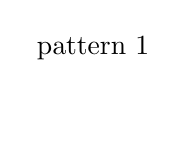
\begin{tikzpicture}
\node [] (n0)  at (0.0,0.0) {};
\node [] (n1)  at (0.0,1.0) {pattern 1}; 
\end{tikzpicture} 
&
\begin{tikzpicture}
\node [] (n1)  at (0.0,2.0) {$T_1 \rightarrow R_1$}; 
\node [] (n2)  at (1.8,1.0) {$T_2 (= R_1) \rightarrow R_3$};
\node [] (n3)  at (4.2,0.0) {$T_3 (= R_2) \rightarrow R_4$}; 

\draw[->] (0.5,1.7) -- (0.5,1.3);
\draw[->] (3.0,0.7) -- (3.0,0.3);


\end{tikzpicture}

\\\hline

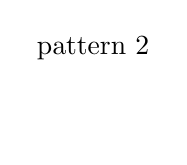
\begin{tikzpicture}
\node [] (n0)  at (0.0,0.0) {};
\node [] (n1)  at (0.0,1.0) {pattern 2}; 
\end{tikzpicture} 
 &
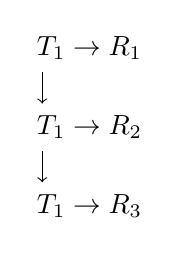
\begin{tikzpicture}
\node [] (n1)  at (0.0,2.0) {$T_1 \rightarrow R_1$}; 
\node [] (n2)  at (0.0,1.0) {$T_1 \rightarrow R_2$};
\node [] (n3)  at (0.0,0.0) {$T_1 \rightarrow R_3$}; 

\draw[->] (-0.6,1.7) -- (-0.6,1.3);
\draw[->] (-0.6,0.7) -- (-0.6,0.3);
\end{tikzpicture}

\\\hline
\begin{tikzpicture}
\node [] (n0)  at (0.0,0.0) {};
\node [] (n1)  at (0.0,2.0) {pattern 3}; 
\end{tikzpicture} 
&
\begin{tikzpicture}
\node [] (n0)  at (2.2,4.0) {$[T]$}; 
\node [] (n1)  at (0.0,3.0) {$T_1 \rightarrow R_1$}; 
\node [] (n2)  at (1.8,2.0) {$T_2 \rightarrow R_2$};
\node [] (n3)  at (4.2,1.0) {$T_3  \rightarrow R_3$}; 

\draw[->] (n0.south) -- (-0.5,3.3);
\draw[->] (n0.south) -- (1.3,2.3);
\draw[->] (n0.south) -- (3.5,1.3);
\end{tikzpicture}

\\\hline

\begin{tikzpicture}
\node [] (n0)  at (0.0,0.0) {};
\node [] (n1)  at (0.0,2.0) {pattern 4}; 
\end{tikzpicture} 
&
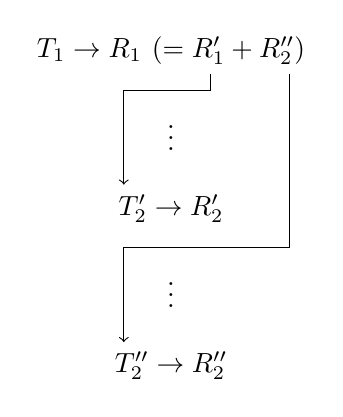
\begin{tikzpicture}
\node [] (n0)  at (0.0,4.0) {$T_1 \rightarrow R_1\textit{ }( = R_1^\prime + R_2^{\prime\prime} )$}; 

\node [] (d0)  at (0.0,3) {$\vdots$}; 

\node [] (n1)  at (0.0,2) {$T_2^\prime \rightarrow R_2^\prime$}; 


\node [] (d0)  at (0.0,1) {$\vdots$}; 


\node [] (n2)  at (0.0,0.0) {$T_2^{\prime\prime} \rightarrow R_2^{\prime\prime}$};

\draw [->] (0.5, 3.7) -- (0.5, 3.5) -- (-0.6, 3.5) -- (-0.6, 2.3);

\draw [->] (1.5, 3.7) -- (1.5, 1.5) -- (-0.6, 1.5) -- (-0.6, 0.3);

\end{tikzpicture}

\end{tabular}
\caption{In the notation used by (?), the horizontal arrow indicates a transition in an utterance, while the vertical one indicates the the contextual connection within of utterances.}
\label{Table:danesh_coherence_patterns}
\end{table}


\newcite{danes74a} interprets the patterns as follows:

\begin{itemize}
\item Pattern 1: A linear transition pattern between themes and rhymes. 
In this pattern, each utterance takes the rhyme presented in the preceding context of the utterance as a given information and transfers it to a new information or a new rhyme. 
In other words, each R (i.e. a new information) becomes the T (i.e. a given information) of the next utterance. 


\item Pattern 2: This pattern depicts a constant theme that continues across utterances. 
One and the same theme appears in a series of utterances. 
Each utterance, however, presents new information about the theme. 


\item Pattern 3: In this pattern $[T]$ indicates a hypertheme that is a global theme of a paragraph or even other text sections. 
 Pattern shows that different utterances can be connected because the themes, or the given information,  of utterances are semantically connected to a hypertheme. 

 \item Pattern 4: 
 \newcite{danes74a} expresses that different combination of these patterns can be employed in different texts. 
 Some of such combinations are so frequent that can be taken as special type of theme-rhyme transition of a higher order. 
  \newcite{danes74a} finds Pattern 4 as one of the most important of such patterns, where an utterance presents two (which can in potential several) rhymes, $R^\prime$ and $R^{\prime\prime}$ , in connection with a given theme. 
  First $R^{\prime}$ expounded and after its progression has been finished, $R^{\prime\prime}$ becomes the theme of another transition. 
  Transitions in between for extending each rhyme follows its own pattern. 
\end{itemize}

\newcite{danes74a} brings this point into attention that one of the important properties of these patterns is omitting links in these patterns.  
For example, in Pattern 1 there is no link between the earliest and latest utterance. 
Those are connected because there is an intermediate utterance that makes transitions between themes and rhymes smoother. 
In contrast, all utterances in Pattern 3  are linked to each other because they all have $T_1$ as a shared given information. 

What \newcite{danes74a} proposed is that the generalized structure of coherent texts may be described in terms of an underlying patterns of transitions between presented themes and rhymes.
This theory is the main motivation of our coherence model in this chapter. 
As before we take entities mentioned in a text as piece of information that make sentences connected. 
The entity graph representation, introduced in Chapter \ref{}, is employed to model the distribution of entities across sentences of a text. 
Then the projection graphs obtained from the entity graph representations of texts model the general structure of sentence node connectivity of texts. 
The entity graph model uses the average ourdegree to encode the connectivity of sentence nodes in projection graphs. 

The main research questions that are investigated in this chapter is:

\begin{itemize}
% \item Is the average outdegree proposed by \newcite{guinaudeau13}  a strong representative metric for the connectivity style of projection graphs and therefore the perceived coherence of texts?
\item Are the any more representative features for the connectivity style of nodes in projection graphs?
\end{itemize}

The idea is to check how well the average outdegree metric models the coherence of a set of well-written articles such as published news articles in Wall Street Journal corpus.  
In spite of this fact that these articles are written by professional authors, human judges assigned to them different range of readability scores (More details in Section \ref{}).  
% We compute the Pearson correlation between the average outdegree of projection graph representations of news articles and their associated score assigned by human judges. 

In order to answer the research question, we employ a subgraph mining algorithm to automatically extract all  subgraphs occurring in projection graphs of these news articles. 
Automatically extracting subgraphs of projection graphs in order to model coherence is our novel contribution in this chapter. 
However, we show that there is a similarity between the automatically mined subgraphs of projection graphs and the coherence patterns proposed by \newcite{danes74a}, indicating that our model's foundation is also linguistically sound.  

We define the frequency of these systematic extracted subgraphs (or coherence patterns) as features that capture the connectivity style of nodes in a projection graph and therefore the coherence property of the corresponding text.  
We evaluate if our novel coherence features outperform the average outdegree feature in a classification task in that more coherent texts should be recognized from less coherent texts. 
In next section, we explain how we exactly model coherence patterns. 


\section{Definitions From Graph Theory}
\label{sec:definition_from_graph_theory}
%
In order to explain the applied subgraphs that encode coherence of sentences in a text, we first need to define some required concepts from graph theory. 

\textbf{Graph.}
A graph is a set of points, we refer to them as nodes, connected by lines, called edges. 
More formally, a graph is a pair of two finite sets $G=( V, E )$ where $V$ is a set of nodes and $E$ is a set of edges whose elements are pairs of nodes. 

\begin{figure}[!ht]
\centering
\small
\begin{tabular}{cc}

	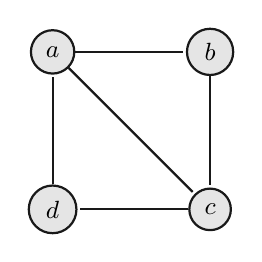
\begin{tikzpicture}[shorten >=1pt,-,scale=0.5]  
		\tikzstyle{node}=[circle,thick,draw=black!90,fill=black!10,minimum size=2mm]
		\tikzstyle{edge}=[draw=black!90, thick]
	   
		 \node [node] (a) at (0,4) {\small{$a$}};
		 \node [node] (b) at (4,4) {\small{$b$}};
		 \node [node] (d) at (0,0) {\small{$d$}}; 
		 \node [node] (c) at (4,0) {\small{$c$}}; 
		 
		 \path[edge] (a) -- (b);
		 \path[edge] (b) -- (c);
		 \path[edge] (c) -- (d);
		 \path[edge] (d) -- (a);
		 \path[edge] (a) -- (c);
       
	\end{tikzpicture}

	&

	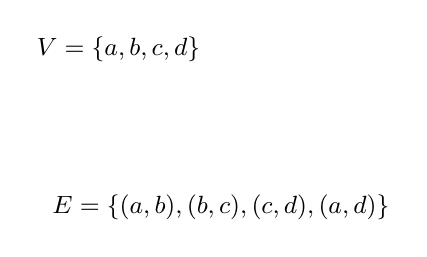
\begin{tikzpicture}[shorten >=1pt,-,scale=0.5]  

		 \node (a) at (0,4) {\small{$V = \left \{ a,b,c,d \right \}$}};
		 \node (b) at (2.6,0) {\small{$E = \left \{(a,b),(b,c),(c,d),(a,d) \right \} $}};

	\end{tikzpicture}

	\\

	$G$ 
	&
	$V:Nodes,E:Edges$ 

\end{tabular}
\caption{Graph. }
\label{fig:graph}
\end{figure} 

If the direction of edges conveys any meaning, then edges can be directed so that for any edge like $e = (x,y)$ the direction is from $x$ towards $y$, which are respectively called the source node and the end node of edge $e$. 
Figure \ref{fig:dir_graph} shows the directed version of the shown graph in Figure \ref{fig:graph}.

\begin{figure}[!ht]
\centering
\small
\begin{tabular}{c}

	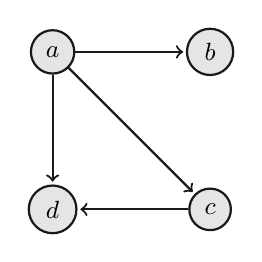
\begin{tikzpicture}[shorten >=1pt,-,scale=0.5]  
		\tikzstyle{node}=[circle,thick,draw=black!90,fill=black!10,minimum size=2mm]
		\tikzstyle{edge}=[draw=black!90, thick]
	   
		 \node [node] (a) at (0,4) {\small{$a$}};
		 \node [node] (b) at (4,4) {\small{$b$}};
		 \node [node] (d) at (0,0) {\small{$d$}}; 
		 \node [node] (c) at (4,0) {\small{$c$}}; 
		 
		 \path[edge,->] (a) -- (b);
		 %\path[edge,->] (b) -- (c);
		 \path[edge,->] (c) -- (d);
		 \path[edge,->] (a) -- (d);
		 \path[edge,->] (a) -- (c);
       
	\end{tikzpicture}
\\

	$G$ 

\end{tabular}
\caption{Directed graph of graph $G$ in Figure \ref{fig:graph}. }
\label{fig:dir_graph}
\end{figure} 


\textbf{Isomorphic.} 
%
Two graphs $G_1$ and $G_2$ are isomorphic, if they fulfill two conditions: (i) a one\--to\--one association, like $f$, exists between nodes of $G_1$ and those of $G_2$, and two nodes of $G_2$ should be connected, if and only if their associated nodes in $G_1$ are connected. 
Figure \ref{fig:isomorphic_graph} illustrates two isomorphic graphs. 
More formally, an isomorphism of graph $G_1$ and $G_2$ is an association between node sets of these graphs:

\begin{equation}
f: V \left( G_1 \right) \rightarrow V \left( G_2 \right),
\end{equation}

such that any  two nodes $u$ and $v$ of $G_1$ are adjacent in $G_1$ if and only if $f \left( u \right)$ and $f \left( v \right)$ are adjacent in $G_2$.
If an isomorphism exists between two graphs, then the graphs are called isomorphic.

\begin{figure}[!ht]
\centering
\small
\begin{tabular}{c@{\hskip 2.5cm}c@{\hskip 2.5cm}c}

	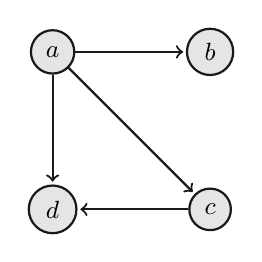
\begin{tikzpicture}[shorten >=1pt,-,scale=0.5]  
		\tikzstyle{node}=[circle,thick,draw=black!90,fill=black!10,minimum size=2mm]
		\tikzstyle{edge}=[draw=black!90, thick]
	   
		 \node [node] (a) at (0,4) {\small{$a$}};
		 \node [node] (b) at (4,4) {\small{$b$}};
		 \node [node] (d) at (0,0) {\small{$d$}}; 
		 \node [node] (c) at (4,0) {\small{$c$}}; 
		 
		 \path[edge,->] (a) -- (b);
		 %\path[edge,->] (b) -- (c);
		 \path[edge,->] (a) -- (c);
		 \path[edge,->] (c) -- (d);
		 \path[edge,->] (a) -- (d);
       
	\end{tikzpicture}

	 &

  	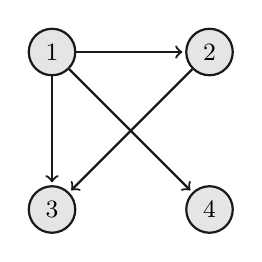
\begin{tikzpicture}[shorten >=1pt,-,scale=0.5]  
	\tikzstyle{node}=[circle,thick,draw=black!90,fill=black!10,minimum size=2mm]
	\tikzstyle{edge}=[draw=black!90, thick]
   
	 \node [node] (1) at (0,4) {\small{$1$}};
	 \node [node] (2) at (4,4) {\small{$2$}};
	 \node [node] (3) at (4,0) {\small{$4$}}; 
	 \node [node] (4) at (0,0) {\small{$3$}}; 
	 
	 \path[edge,->] (1) -- (2);
	 \path[edge,->] (1) -- (3);
	 \path[edge,->] (1) -- (4);
	 \path[edge,->] (2) -- (4);
   
  \end{tikzpicture}

	 &

  	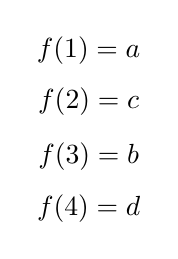
\begin{tikzpicture}[shorten >=1pt,-,scale=0.5]  

	 \node  (1) at (0,4) {$f(1) = a$};
	 \node  (2) at (0,2.7) {$f(2) = c$};
	 \node  (3) at (0,1.3) {$f(3) = b$}; 
	 \node  (4) at (0,0) {$f(4) = d$}; 

  \end{tikzpicture}
\\
$ G_1 $ 
&
 $G_2$
& 
$\textit{Node associations}$

\end{tabular}
\caption{Two isomorphic graphs and a sample association between their nodes. }
\label{fig:isomorphic_graph}
\end{figure} 


\textbf{Subgraph.} 
%
Graph $G_2$ is a subgraph of graph $G_1$, if $G_2$ is isomorphic to a graph whose nodes and edges are a subset of nodes and edges of $G_1$.
\begin{figure}[!ht]
\centering
\small
\begin{tabular}{c@{\hskip 2.5cm}c@{\hskip 2.5cm}c}

	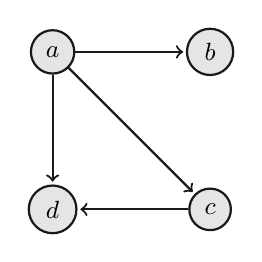
\begin{tikzpicture}[shorten >=1pt,-,scale=0.5]  
		\tikzstyle{node}=[circle,thick,draw=black!90,fill=black!10,minimum size=2mm]
		\tikzstyle{edge}=[draw=black!90, thick]
	   
		 \node [node] (a) at (0,4) {\small{$a$}};
		 \node [node] (b) at (4,4) {\small{$b$}};
		 \node [node] (d) at (0,0) {\small{$d$}}; 
		 \node [node] (c) at (4,0) {\small{$c$}}; 
		 
		 \path[edge,->] (a) -- (b);
		 %\path[edge,->] (b) -- (c);
		 \path[edge,->] (a) -- (c);
		 \path[edge,->] (c) -- (d);
		 \path[edge,->] (a) -- (d);

       
	\end{tikzpicture}

	 &

  	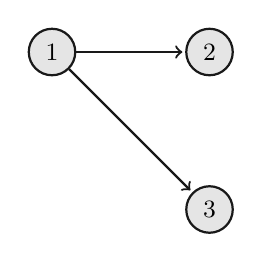
\begin{tikzpicture}[shorten >=1pt,-,scale=0.5]  
	\tikzstyle{node}=[circle,thick,draw=black!90,fill=black!10,minimum size=2mm]
	\tikzstyle{edge}=[draw=black!90, thick]
   
	 \node [node] (1) at (0,4) {\small{$1$}};
	 \node [node] (2) at (4,4) {\small{$2$}};
	 \node [node] (3) at (4,0) {\small{$3$}}; 
	 
	 \path[edge,->] (1) -- (2);
	 \path[edge,->] (1) -- (3);
   
  \end{tikzpicture}

	 &

  	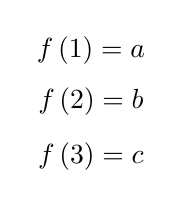
\begin{tikzpicture}[shorten >=1pt,-,scale=0.5]  

	 \node  (1) at (0,4) {$f \left( 1 \right) = a$};
	 \node  (2) at (0,2.7) {$f \left( 2 \right) = b$};
	 \node  (3) at (0,1.3) {$f \left( 3 \right) = c$}; 

  \end{tikzpicture}
\\
$ G_1 $ & $G_2$  & $\textit{Node associations}$

\end{tabular}
\caption{$G_2$ is a subgraphs of graph $G_1$}
\label{fig:subgraph}
\end{figure} 

In the shown example in Figure \ref{fig:subgraph}, graph $G_2$ is isomorphic with graph 

\begin{equation}
G = \left( \left\{ a,b,c \right\}, \left\{ \left( a , b \right),\left( b , c \right) \right\} \right) 
\end{equation}

whose node and edge sets are subsets of node and edge sets of $G_1$.

\textbf{k-node subgraph.}
%
The size of subgraph is the size of its node set that is the number nodes in the graph. 
Graph $G_2 = \left( V_2 , E_2 \right)$ is a k-node subgraph of graph $G_1 = \left( V_1, E_1 \right)$, if $G_2$ is a subgraph of $G_1$, and $V_2$ has $k$ elements, $|V_2|=k$. 
In Figure \ref{fig:subgraph}, graph $G_2$ is a 3-node subgraph of graph $G_1$. 


\textbf{Induced subgraph.} 
%
An induced subgraph of a graph is a subgraph of the graph with an extra condition on its edges.  
That is, in simple words, its edge sets contains all possible edges that are present in the main graph. 
Formally, graph $G_2 = (V_2, E_2)$ is an induced subgraph of graph $G_1 = (V_2, E_2)$ if $V_2 \subseteq V_1$ and 
\begin{equation}
E_2 = \left\{ (x,y)| x \in V_2, y \in V_2, (x,y) \in E_1   \right\}. 
\end{equation}

Figure \ref{fig:induced_subgraphs} shows a graph and two subgraphs of it. 
Subgraph $G_2$ is a subgraph of $G_1$ but not induced, because there is no edge between nodes $1$ and $3$ of this subgraph while their associated nodes, $a$ and $b$, in graph $G_1$ are connected. 
In contrast, subgraph $G_2$ is an induced subgraph of $G_1$ because it contains all possible edges that are present in $G_1$ and connect nodes of the subgraph.  

\begin{figure}[!ht]
\centering
\small
\begin{tabular}{c@{\hskip 1.5cm}c@{\hskip 1.5cm}c@{\hskip 1.5cm}c}

	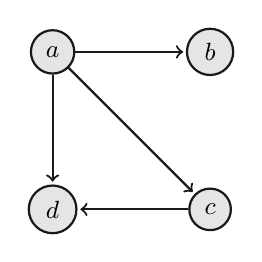
\begin{tikzpicture}[shorten >=1pt,-,scale=0.5]  
		\tikzstyle{node}=[circle,thick,draw=black!90,fill=black!10,minimum size=2mm]
		\tikzstyle{edge}=[draw=black!90, thick]
	   
		 \node [node] (a) at (0,4) {\small{$a$}};
		 \node [node] (b) at (4,4) {\small{$b$}};
		 \node [node] (d) at (0,0) {\small{$d$}}; 
		 \node [node] (c) at (4,0) {\small{$c$}}; 
		 
		 \path[edge,->] (a) -- (b);
		 \path[edge,->] (a) -- (c);
		 \path[edge,->] (c) -- (d);
		 \path[edge,->] (a) -- (d);

       
	\end{tikzpicture}

	 &

  	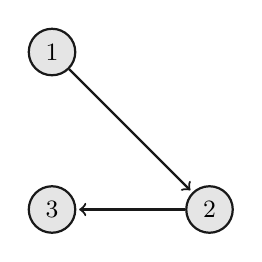
\begin{tikzpicture}[shorten >=1pt,-,scale=0.5]  
	\tikzstyle{node}=[circle,thick,draw=black!90,fill=black!10,minimum size=2mm]
	\tikzstyle{edge}=[draw=black!90, thick]
   
	 \node [node] (1) at (0,4) {\small{$1$}};
	 \node [node] (2) at (4,0) {\small{$2$}};
	 \node [node] (3) at (0,0) {\small{$3$}}; 
	 
	 \path[edge,->] (1) -- (2);
	 \path[edge,->] (2) -- (3);
   
  \end{tikzpicture}

	 &


  	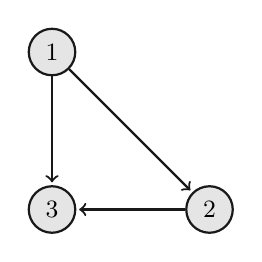
\begin{tikzpicture}[shorten >=1pt,-,scale=0.5]  
	\tikzstyle{node}=[circle,thick,draw=black!90,fill=black!10,minimum size=2mm]
	\tikzstyle{edge}=[draw=black!90, thick]
   
	 \node [node] (1) at (0,4) {\small{$1$}};
	 \node [node] (2) at (4,0) {\small{$2$}};
	 \node [node] (3) at (0,0) {\small{$3$}}; 
	 
	 \path[edge,->] (1) -- (2);
	 \path[edge,->] (2) -- (3);
	 \path[edge,->] (1) -- (3);
   
  \end{tikzpicture}

  &

  	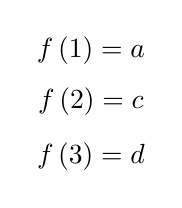
\begin{tikzpicture}[shorten >=1pt,-,scale=0.5]  

	 \node  (1) at (0,4) {$f \left( 1 \right) = a$};
	 \node  (2) at (0,2.7) {$f \left( 2 \right) = c$};
	 \node  (3) at (0,1.3) {$f \left( 3 \right) = d$}; 

  \end{tikzpicture}
\\
$ G_1 $ & $G_2$  & $G_3$ & $\textit{Node associations}$

\end{tabular}
\caption{Induced subgraphs}
\label{fig:induced_subgraphs}
\end{figure} 

It is worth mentioning that henceforth we mean induced subgraphs when using the term subgraph.  
However, in cases that the context is not clear we explicitly distinguish them.     


\textbf{Graph signature.} 
%
Given a list of graphs $ \zeta  = \left[ G_1, G_2, \cdots , G_m \right]$,  a graph signature, which is  denoted by for graph $G$, denoted by $\phi \left( G \right)$,  with respect to $\zeta$ is a vector of frequencies of graphs in $\zeta$ in graph $G$:

\begin{equation}
\phi \left( G \right) = \left( f_1, f_2, f_3, \cdots, f_m \right),
\end{equation}
%
where $f_i$ is the frequency of graphs in graph $G$. 
The frequency of graph $G_i$ in graph $G$ is computed as follows:

\begin{equation}
 f_i = \frac{count(G_i, G)}{\sum_{G_j \in \zeta}{count(G_j, G)}}
\end{equation}
%
where $count(G_i, G)$ is the number of occurrences of $G_i$ in graph $G$. 
The reason of using frequency instead of raw count is that frequency is a normalized value that cannot become biased to the number of nodes and edges of graph $G$. 



\section{Coherence Patterns Modeling}
\label{sec:coherence_patterns_modeling}
%
The entity graph representation of a text encodes the distribution of entities across sentences of a text. 
One-mode projection graphs model the connectivity between sentence nodes with respect to the shared entities between sentences. 
Our main contribution, in this chapter, is that instead of the average outdegree as a simple metric that models the connectivity of sentence nodes of a projection graph, we introduce a set of novel graph-based features that encode the structure of connections (i.e.\ connectivity style) in a projection graph. 
We hypothesize that the frequencies of different subgraphs occurring in projection graphs encode the connectivity style of  projection graphs and therefore, they can be utilized to model coherence.  
Our experiments in Section \ref{} indicate this hypothesis is correct for the examined tasks.  

Given a corpus of documents, we model connections between sentences of each document by its projection graph representation, $P_U$. 
In this step, instead of having a set of documents we have a set of one-mode projection graphs associated with documents. 
We refer to it as the graph set.  
Similar to the entity grid model \cite{barzilay08b}, the key assumption behind our coherence model is that coherent texts reveal similar patterns that differ them from incoherent texts. 
Therefore, the projection graphs of coherent texts reveal similar connectivity style that is different with incoherent texts. 
\newcite{guinaudu13} propose the average outdegree, but we propose to use the graph signature of each projection graph to encode the connectivity style of projection graphs into a vector. 

In order to obtain graph signatures of projection graphs, some basis graphs are required to represent projection graphs based on them. 
We propose to extract all possible subgraphs of projection graphs as basis graphs for computing graph signatures. 

The results of our experiments in Section \ref{}, show that the frequencies of some subgraphs in documents are statistically significantly correlated with scores assigned by human annotators to documents. 
Moreover, as it will be shown in Section \ref{}, some of these subgraphs are similar to what are defined by \newcite{danes74a}. 
Considering these all, we refer to these subgraphs coherence patterns and their frequencies as coherence features.  

Figure \ref{} shows a schema of our idea for extracting coherence patterns and features. 

From the machine learning perspective, the vector representation of the projection graphs can be taken as feature vectors, in which each element is a feature representing one aspect of data. 
These feature vectors can be supplied to any machine learning model in order to classify coherent documents from incoherent documents. 

\subsection{Subgraph Mining: gSpan Method}
\label{subsec:subgraph_mining_gspan}
%
Coherence patterns are subgraphs that occur at least in one of projection graphs of documents in a corpus. 
Mining all subgraphs that occur in a graph set is computationally expensive and this problem is proved to be an NP-complete problem \cite{}. 
Intuitively, a graph with $\Vert E \Vert$ edges, potentially has $\mathcal{O} \left( 2^{\Vert E \Vert} \right)$ subgraphs.  
Projection graphs with $\Vert V \Vert$ nodes at most has  $\frac{(\Vert V \Vert-1)(\Vert V \Vert-2)}{2}$ that is in order of $\mathcal{O} \left( \Vert V \Vert ^2 \right)$.  

In general, the goal of this thesis is not to develop an algorithm for subgraph mining. 
This has been widely studied in computer science and different algorithms and packages have been developed for this. 
The gSpan\footnote{We use the Java package: \url{http://www.cs.ucsb.edu/~xyan/software/gSpan.htm}}  algorithm \cite{yanxifeng02} is one of the efficient methods for mining subgraphs of a  graph set. 
Here, we briefly describe the idea and the method of the gSpan algorithm and refer interested readers to Appendix \ref{} for more details. 

The gSpan,(\textit{g}raph-based \textit{S}ubstructure \textit{pa}ttern \textit{m}ining), algorithm is an approach for extracting all patterns (i.e. subgraphs) that frequently occur in a graph set. 
It discovers all frequent subgraphs without generating the candidates. 
So it is more efficient. 
A subgraph is called frequent if the number of graphs that contain the subgraph is greater than a threshold. 
This threshold is a hyper-parameter of the algorithm\footnote{We always set this threshold to zero to extract all occurring subgraphs in a graph set. We prefer all patterns over frequent patterns because our goal is to investigate .....
 However, is it possible to integrate this in the future work?}.
 gSpan orders graphs in a graph set with respect to their structures and then adapts a depth-first-search search strategy to extract frequent connected subgraphs efficiently. 
 It starts with small subgraphs and simultaneously expands subgraphs and check the frequency of subgraph. 

\textbf{
 [It seems the efficiency of gSpan is when you have a threshold, by setting this to zero it has to extract all possible patterns, so the method is still expensive..]
}


\section{Coherence Modeling}
\label{sec:automatic_extraction}
%
Given a corpus of documents, we employ the entity graph to represent the entity distribution between sentences of each document in the corpus. 
We apply a one-mode projection on each entity graph to obtain an unweighted projection graph (i.e. $P_U$) over the sentence nodes of the entity graph. 
$P_U$ models the overall entity-based connectivity among sentences of a document. 
We extract all possible k-node subgraphs (i.e. coherence patterns) that occur in the projection graphs associated to documents in the corpus. 
k is a parameter of the model that controls the size of subgraphs. 
Controlling the size of subgraphs mainly helps to run the subgraph mining algorithm more efficiently in terms of computational time and number of subgraphs. 
More over, small subgraphs are more likely to occure in larger subgraphs. 
Therefore consdering subgraphs with different sizes result in subgraphs whose frequencies might be correlated. 
These type of features are advised to be split up in machine learning methods. 

Assuming that $m$ coherence patterns are mined from all projection graphs, the coherence of a document is encoded as a vector of frequencies of the $m$ mined patterns in the projection graph representation of the document. 
Therefore the coherence of a document, $d$, will be represented by a vector as follows:

\begin{equation}
<f_0,f_1,f_2,...,f_m>
\end{equation}
%
where $f_i$ represents the frequency of the $i^{th}$ pattern, out of $m$ mined patterns, in the projection graph representation of document $d$. 

Similar to what is explained in the entity grid model \cite{barzilay08b}, these feature vectors can be employed by machine learning models in two ways. 
A machine learning model during training learns to map feature vectors to  scores, which can be interpreted as coherence scores, such that scores of  coherent texts be higher than those of incoherent ones. 
More formally, given two documents $d$ and $d^\prime$ where $d$ is more coherent than $d^\prime$, then 

\begin{equation}
\beta ( d_v) > \beta (d^\prime_v)
\end{equation}
%
where $d_v$ and $d^\prime_v$ are the feature vectors representing the coherence property of these documents, and $\beta$ is a paramateric function whose parameters are trained by a machine learning model like Support Vector Machine (SVM).


\subsection{Coherence Patterns}
\label{subsec:coherence_patterns}
%
As we explained above, we limit the size of extracted subgraphs from all projection graphs by defining parameter k that is the number of nodes in subgraphs. 

In this chapter, we investigate the usefulness of these patterns for coherence modeling. 
We limit the size of coherence patterns to sets of subgraphs. 
One set consists of subgraphs that has three nodes, henceforth 3-node subgraphs, the other set contains subgraphs with four nodes, we refer to them 4-node subgraphs. 
There is not any criteria on the number of edges in subgraphs, except that the subgraphs should be connected. 

We begin with extracting 3-node subgraphs in order to examine the soundness of mined coherence patterns.  
3-node subgraphs are the smallest meaningful patterns that can model the connectivity style of sentence nodes in projection graphs. 
There is only one 2-node subgraph, ($\lbrace a,b \rbrace,\lbrace \left( a, b\right) \rbrace$), that its frequency is the number of edges in each projection graph that has the same interpretation as the average outdegree applied by the entity graph model.  
We believe that if the connectivity style of projection graphs of coherent texts are similar to each other and different with projection graphs of incoherent texts, 3-node subgraphs should capture this. 
This hypothesis is evaluated in Section \ref{}.

However, 3-node subgraphs are too small and they are likely to occur in most projection graphs in a graph set. 
We hypothesis that larger subgraphs better captures the connectivity style of projection graphs than the 3-node subgraphs, while 3-node subgraphs are easier for interpretation. 
In this chapter, we extract 4-node subgraphs to have a better representation of the connectivity style of projection graphs. 
Our experiments in Section \ref{} evaluates our hypothesis in this part, that is larger subgraphs, specifically 4-node subgraphs, are better representative for connectivity of nodes of projection graphs and therefore the perceived coherence of texts in corpus in comparison with 3-node subgraphs.


\section{Experiments}
\label{sec:experiments}
%
In this section, we evaluate three-fold:
\begin{itemize}
	\item How well average outdegree, the coherence metric defined in the entity graph model, does encode coherence?
	\item How valid is our assumption that the frequencies of our smallest coherence patterns, i.e. 3-node subgraphs, contribute to coherence modeling?
	\item How valid is this assumption that 4-node coherence patterns better represent the connectivity style of the projection graphs and therefore coherence in comparison with 3-node subgraphs?
	\item Are these novel coherence patterns and their frequencies as coherence features better predictive than the average outdegree for coherence?
\end{itemize}

As we discussed in Chapter \ref{}, coherence is better to be evaluated in an extrinsic fashion. 
It is mainly because annotating texts for coherence is quite expensive and controlling all conditions for annotators is very difficult. 
In this chapter, we focus on two extrinsic evaluation tasks: readability assessment and automatic text summarization. 
The former one is used to evaluate the predictive power of different proposed coherence features by computing the correlation between the values of the coherence features and the readability scores assigned by human judges. 
We also check how well coherence features can rank documents with respect to their readability level. 
The latter task is a specific instance of text generation, where a subset of informative sentences in a document should be extracted and presented in a proper order to generate a coherence and readable summary. 
In this experiment, we evaluate the capabilities of our coherence patterns in producing coherent summaries. 
We show that by integrating our coherence patterns into a graph-based document summarizer \cite{parveen15}, the performance of the summarizer improves in terms of ROUGE metrics and human qualitative evaluations.

\subsection{Readability Assessment}
\label{subsec:readability_assessment}
%
Readability assessment is about how well a text is understandable for its readers? 
It is a challenging problem because various factors affect the processing time of a text for its readers including both text properties (such as syntactic and semantic features) and reader's abilities (e.g., the background knowledge of readers). 
Possible applications of readability assessment are automatic text summarization and simplification systems. 
Measuring readability can also be used in question answering and knowledge extraction systems to prune texts with low readability \cite{kate10}.
Obviously, Many different text features can be used to assess readability including shallow features \cite{flesch48,kincaid75}, language modeling features \cite{siluo01,collins-thompson04}, syntactic features \cite{schwarm05} and text flow or coherence \cite{barzilay08,pitler08}.
In this work, the readability assessment task  basically investigates the application of coherence features to quantify the difficulty of text understanding.  
In a coherent text each sentence has some connections with other sentences. 
Although these local connections make texts easier to read, the coherence features introduced by the entity grid model \cite{barzilay08b} and evaluated in \newcite{pitler08} are not strongly correlated with human judgments. 
It has been shown that the entity graph representations of entities across sentences of texts better encode the entity-based relations between sentences (More details in  chapter \ref{}). 
Here, we investigate if the average outdegree metric, and our coherence features that are defined based on the entity graph representations of texts are correlated with human readability judgments. 

Here, we need to emphasis that readability is beyond coherence. 
This is why we do not use coherence features to predict the  readability scores associated with documents. 
However, because coherence is one of the crucial factors in readability assessment, easier-to-read texts imply to be more coherent as well. 
We expect that the values of coherence features show a strong correlation with readability scores associated to documents. 
In another experiment, we also check how well we can rank documents with respect to their readability if only coherence has been taken into account. 

\subsubsection{Data}
%
We use the dataset created by \newcite{pitler08} which consists of thirty randomly selected articles from the Wall Street Journal corpus intended for an educational adult audience. 

We exclude three articles from the dataset. 
One article is poem and is removed in order to analyze articles with the same style. 
Two other articles are missing in the new versions of Penn Discourse Treebank.
The complete list of article IDs and their associated readability scores are presented in Appendix \ref{}.
% : \texttt{wsj\--0382} does not exist in the Penn Treebank \cite{marcus94}. 
% \newcite{pitler08} also remove one file from their experiments. 
% We assume that it is  \texttt{wsj\--0382}.}. 
% \texttt{wsj\--2090} does not exist in the Penn Discourse Treebank \cite{prasad08a}. 
% \texttt{wsj\--1398} is a also poem.


The articles were rated by three human judges on a scale from $1$ to $5$, higher is better, for readability based on quality measures that are designed to estimate the coherence of articles. 
Each judges was given unlimited time to read the texts and perform the ratings. 
Human judges received following questions \cite{pitler08}:
\begin{itemize}
	\item How well-written is this article?
	\item How well does the text fit together?
	\item How easy was it to understand?
	\item How interesting is this article?
\end{itemize} 
 
\newcite{pitler08} explain that since most of the time judges gave the same rating to all questions, they only consider the given rates for the first question (How well-written is this article) and then the average if rates are taken as the final score. 
This is the reason that they use this scores for coherence evaluations as well \cite{pitler08}.  
The final readability score of each article is the average of these three ratings.

This dataset is more realistic than the one used in the previous chapter for predicting readability level.  
Mainly because these articles appeared in the Wall Street Journal and are aimed at the same target audience. 

\textbf[Do you have some statistics about the dataset. If so put it here. Read Pitler and Nenkova paper for one more time. You can also add a text from the corpus and its associated score. ].



\subsubsection{Feature Analysis}
\label{subsubsec:feature_analysis}
%
The goal of this experiment is to investigate the correlation of different coherence features with coherence features are correlated with the associated readability scores with the articles. 
To this end, we represent each article in the dataset by its entity graph, where entities are obtained heuristically by string match between all nouns in articles. 
We apply a one-mode projection to obtain unweighted projection graphs. 
This projection graph models the entity-based connectivity between sentences of articles. 
Given the corresponding projection graphs of articles in corpus, we compute the Pearson correlation between the value of a feature and associated readability scores to articles. 

The Pearson correlation coefficient is a measure of the linear correlation between values of two variables. 
Here variables are a coherence feature and the readability ratings assigned to articles by humans. 
The Pearson correlation coefficient, $\rho$, ranges between $-1$ and $+1$ where a high absolute value of $\rho$ shows a strong correlation between variables. 
The sign of $\rho$ indicates the direction of relationships between examined variables. 
In extreme cases, $+1$ shows a total positive linear correlation, $0$ is no linear correlation, and $-1$ is total negative linear correlation. 
The Pearson correlation also measures how statistically significant examined variables are correlated. 
This measure is referred to by $p_{value}$. 
We consider correlations with $p_{value} < 0.01$ statistically significant. 
Appendix \ref{} explains more mathematical details of Pearson correlation.

We compare following features with each others: average outdegree, the number of components in projection graphs, frequencies of 3-node patterns, frequencies of 4-node patterns. 



\paragraph{Implementation Details.} In order to be compatible with the entity grid features that are used by \newcite{pitler08}, we also use the gold parse trees in the Penn Treebank (Marcus et al., 1994) to extract all nouns in an  article as mentions. 
All nouns with identical stems are taken coreferent. 

\textbf{[TO DO. DO you use brown coherence toolkit? Did you implement this in JAVA?]}

We used the a Java implementation of the gSpan algorithm that is publicly available\footnote{http://www.cs.ucsb. edu/\~xyan/software/gSpan.htm}. 
This package counts all subgraphs regardless of this fact that a subgraph is induced or not. 
Since we are interested in only subgraphs we employed sage-Math\footnote{\url{http://sagemath.org/download- linux.html}} for graph processing. 
Induced subgraphs counting is done by this package. 
For computing the correlation between feature values and readability scores we use the Pearson correlation implemented in ``scipy'' package in python 2.7. 


\paragraph{Mined Coherence Patterns.} 
Figure \ref{fig:feasible_3node_subgraphs} shows mined coherence patterns with three nodes. 
\begin{figure}[!t]
\centering
\resizebox{1.0\columnwidth}{!}{
\begin{tabular}{@{}c@{\hskip 1.5cm}c@{\hskip 1.5cm}c@{\hskip 1.5cm}c@{}}
 %%%%%%%%%%%%%%%%%%%%%%%%%%%%%% subgraph 1 %%%%%%%%%%%%%%%%%%%%%%%%%%%%%%
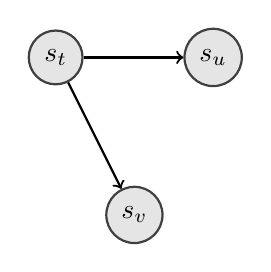
\begin{tikzpicture}  
        \tikzstyle{sentence}=[circle,thick,draw=black!75,fill=black!10,minimum size=5mm]
        \tikzstyle{edge}=[draw, thick]
       \begin{scope}
         \node [sentence] (s1) at (0,2) {$s_t$};
         \node [sentence] (s2) at (2,2) {$s_u$};
         \node [sentence] (s3) at (1,0) {$s_v$}; 
         \path[edge,->] (s1) edge  (s2);
         \path[edge,->] (s1) edge  (s3);
        \end{scope}        
      \end{tikzpicture}
&
%%%%%%%%%%%%%%%%%%%%%%%%%%%%%% subgraph 2 %%%%%%%%%%%%%%%%%%%%%%%%%%%%%%
 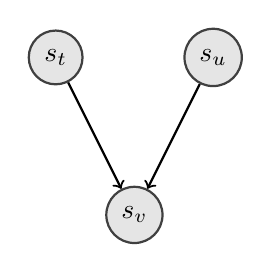
\begin{tikzpicture} 
        \tikzstyle{sentence}=[circle,thick,draw=black!75,fill=black!10,minimum size=5mm]
        \tikzstyle{edge}=[draw, thick]
       \begin{scope}
         \node [sentence] (s1) at (0,2) {$s_t$};
         \node [sentence] (s2) at (2,2) {$s_u$};
         \node [sentence] (s3) at (1,0) {$s_v$}; 
         \path[edge,->] (s1) edge  (s3);
         \path[edge,->] (s2) edge (s3);
        \end{scope}        
      \end{tikzpicture}

&
 %%%%%%%%%%%%%%%%%%%%%%%%%%%%%% subgraph 3 %%%%%%%%%%%%%%%%%%%%%%%%%%%%%%
 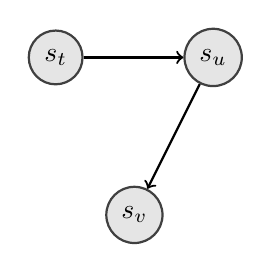
\begin{tikzpicture}
        \tikzstyle{sentence}=[circle,thick,draw=black!75,fill=black!10,minimum size=5mm]
        \tikzstyle{edge}=[draw, thick]
       \begin{scope}
         \node [sentence] (s1) at (0,2) {$s_t$};
         \node [sentence] (s2) at (2,2) {$s_u$};
         \node [sentence] (s3) at (1,0) {$s_v$}; 
         \path[edge,->] (s1) edge (s2);
         \path[edge,->] (s2) edge (s3);
        \end{scope}        
      \end{tikzpicture}
      
      
 &
 %%%%%%%%%%%%%%%%%%%%%%%%%%%%%% subgraph 7 %%%%%%%%%%%%%%%%%%%%%%%%%%%%%%
 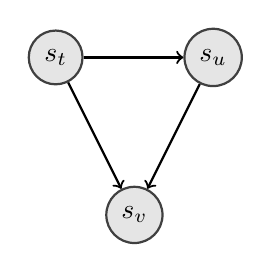
\begin{tikzpicture}  
        \tikzstyle{sentence}=[circle,thick,draw=black!75,fill=black!10,minimum size=5mm]
        \tikzstyle{edge}=[draw, thick]
       \begin{scope}
        \node [sentence] (s1) at (0,2) {$s_t$};
         \node [sentence] (s2) at (2,2) {$s_u$};
         \node [sentence] (s3) at (1,0) {$s_v$};
         \path[edge,->] (s1) edge (s2);
         \path[edge,->] (s1) edge (s3);
         \path[edge,->] (s2) edge (s3);
         
        \end{scope}        
      \end{tikzpicture} 
\\

$sg_1$& $sg_2$ & $sg_3$ & $sg_4$
\end{tabular}
}
\caption{Feasible 3\--node subgraph coherence features.}
\label{fig:feasible_3node_subgraphs}
\end{figure}
%
We interpret these patterns as follows:
\begin{itemize}
\item \boldmath{$sg_1$}\textbf{:} 
A sentence is connected with two subsequent sentences.
More precisely, at least two entities are mentioned in one sentence and the subsequent ones are about these entities.

\item \boldmath{$p_2$}\textbf{:} 
The connection between two sentences is made by a sentence that comes after those sentences. 
This patterns indicates that entities in $s_t$ and $s_u$ are connected to each other in $s_v$. 

\item \boldmath{$sg_3$}\textbf{:} 
Each sentence tends to refer to the most prominent entity (the focus of attention) in preceding sentences \cite{sidner83,grosz95}. 
The absence of a connection between $s_t$ and $s_v$ indicates that the entity connecting $s_t$ and $s_u$ is different from the entity connecting $s_u$ and $s_v$. 
Therefore this subgraph approximately corresponds to the shift of the focus of attention.
This pattern explains why we use induced subgraphs as coherence patterns. 

\item \boldmath{$sg_4$}\textbf{:} 
This pattern encodes three sentences that all are connected with each other. 
Entities that connect sentences are not necessarily unique. 
An important property of this pattern is that it has maximum number of edges showing many  repetitions of entities in sentences. 
\end{itemize}

We take these 3-node subgraphs as coherence patterns and compute the graph signature, $\Phi$, of each projection graph corresponding with each document in a dataset. 
The elements of a graph signature are frequencies of the extracted subgraphs in the graph. 
These elements together model the connectivity style of the graph. 
From texture perspective, the frequency of each subgraphs models how frequently a coherence pattern is used in a text. 
We hypothesize that the frequency of some patterns in coherent texts are greater than those in incoherent ones. 
At the same time some patterns are expected be less frequent in coherent texts than coherent ones. 

 
We also hypothesize that 4-node subgraphs are more informative coherence patterns, because they are larger than 3-node subgraphs and they can capture more information about the connectivity style of projection graphs. 
In addition, 4-node subgraphs are less likely to occur in all projection graphs.
So their frequencies are expected to better distinguish between coherent and incoherent texts.   
Another advantage of coherence patterns is that using these patterns coherence can be measured beyond simple sentence or node connectivity. 
This is one of the essential differences between our coherence patterns and average ourdegree \cite{}.

Figure \ref{} shows all mined subgraphs from the projection graphs corresponding to documents in readability dataset. 

\begin{figure}[!t]
\centering
\begin{tabular}{@{}c@{\hskip 1.5cm}c@{\hskip 1.5cm}c@{\hskip 1.5cm}c@{}}
\scriptsize{$sg_1$} & \scriptsize{$sg_2$} & \scriptsize{$sg_3$} & \scriptsize{$sg_4$}
\\
 %%%%%%%%%%%%%%%%%%%%%%%%%%%%%% sg 1 = 73 %%%%%%%%%%%%%%%%%%%%%%%%%%%%%%
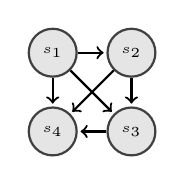
\begin{tikzpicture}[shorten >=1pt,->,scale=0.5]  
        \tikzstyle{sentence}=[circle,thick,draw=black!75,fill=black!10,minimum size=1mm]
        \tikzstyle{edge}=[draw, thick]
       \begin{scope}
         \node [sentence] (s1) at (0,2) {\tiny{$s_1$}};
         \node [sentence] (s2) at (2,2) {\tiny{$s_2$}};
         \node [sentence] (s3) at (2,0) {\tiny{$s_3$}};
         \node [sentence] (s4) at (0,0) {\tiny{$s_4$}};  
         \path[edge] (s1) edge [above] node[font=\tiny] {} (s2);
         \path[edge] (s1) edge [above] node[font=\tiny] {} (s3);
         \path[edge] (s1) edge [above] node[font=\tiny] {} (s4);
         \path[edge] (s2) edge [above] node[font=\tiny] {} (s4);
         \path[edge] (s2) edge [above] node[font=\tiny] {} (s3);
         \path[edge] (s3) edge [above] node[font=\tiny] {} (s4);
        \end{scope}        
      \end{tikzpicture}
&
%%%%%%%%%%%%%%%%%%%%%%%%%%%%%% sg 2 = 74 %%%%%%%%%%%%%%%%%%%%%%%%%%%%%%
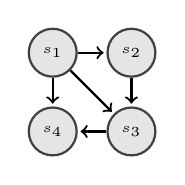
\begin{tikzpicture}[shorten >=1pt,->,scale=0.5]  
        \tikzstyle{sentence}=[circle,thick,draw=black!75,fill=black!10,minimum size=2mm]
        \tikzstyle{edge}=[draw, thick]
       \begin{scope}
         \node [sentence] (s1) at (0,2) {\tiny{$s_1$}};
         \node [sentence] (s2) at (2,2) {\tiny{$s_2$}};
         \node [sentence] (s3) at (2,0) {\tiny{$s_3$}};
         \node [sentence] (s4) at (0,0) {\tiny{$s_4$}};  
         \path[edge] (s1) edge [above] node[font=\tiny] {} (s2);
         \path[edge] (s1) edge [above] node[font=\tiny] {} (s3);
         \path[edge] (s1) edge [above] node[font=\tiny] {} (s4);
         \path[edge] (s2) edge [above] node[font=\tiny] {} (s3);
         \path[edge] (s3) edge [above] node[font=\tiny] {} (s4);
        \end{scope}        
      \end{tikzpicture}
&
%%%%%%%%%%%%%%%%%%%%%%%%%%%%%% sg 3 = 83 %%%%%%%%%%%%%%%%%%%%%%%%%%%%%%
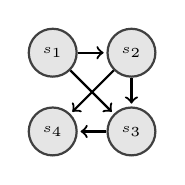
\begin{tikzpicture}[shorten >=1pt,->,scale=0.5]  
        \tikzstyle{sentence}=[circle,thick,draw=black!75,fill=black!10,minimum size=2mm]
        \tikzstyle{edge}=[draw, thick]
       \begin{scope}
         \node [sentence] (s1) at (0,2) {\tiny{$s_1$}};
         \node [sentence] (s2) at (2,2) {\tiny{$s_2$}};
         \node [sentence] (s3) at (2,0) {\tiny{$s_3$}};
         \node [sentence] (s4) at (0,0) {\tiny{$s_4$}};  
         \path[edge] (s1) edge [above] node[font=\tiny] {} (s2);
         \path[edge] (s1) edge [above] node[font=\tiny] {} (s3);
         \path[edge] (s2) edge [above] node[font=\tiny] {} (s3);
         \path[edge] (s2) edge [above] node[font=\tiny] {} (s4);
         \path[edge] (s3) edge [above] node[font=\tiny] {} (s4);
        \end{scope}        
      \end{tikzpicture}
&
%%%%%%%%%%%%%%%%%%%%%%%%%%%%%% sg 4 =84 %%%%%%%%%%%%%%%%%%%%%%%%%%%%%%
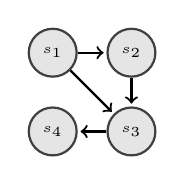
\begin{tikzpicture}[shorten >=1pt,->,scale=0.5]  
        \tikzstyle{sentence}=[circle,thick,draw=black!75,fill=black!10,minimum size=2mm]
        \tikzstyle{edge}=[draw, thick]
       \begin{scope}
         \node [sentence] (s1) at (0,2) {\tiny{$s_1$}};
         \node [sentence] (s2) at (2,2) {\tiny{$s_2$}};
         \node [sentence] (s3) at (2,0) {\tiny{$s_3$}};
         \node [sentence] (s4) at (0,0) {\tiny{$s_4$}};  
         \path[edge] (s1) edge [above] node[font=\tiny] {} (s2);
         \path[edge] (s1) edge [above] node[font=\tiny] {} (s3);
         \path[edge] (s2) edge [above] node[font=\tiny] {} (s3);
         \path[edge] (s3) edge [above] node[font=\tiny] {} (s4);
        \end{scope}        
      \end{tikzpicture}
\\
\scriptsize{$sg_5$} & \scriptsize{$sg_6$} & \scriptsize{$sg_7$} & \scriptsize{$sg_8$}
\\
%%%%%%%%%%%%%%%%%%%%%%%%%%%%%% sg 5 = 106 %%%%%%%%%%%%%%%%%%%%%%%%%%%%%%
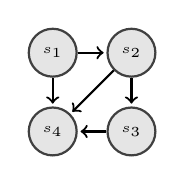
\begin{tikzpicture}[shorten >=1pt,->,scale=0.5]  
        \tikzstyle{sentence}=[circle,thick,draw=black!75,fill=black!10,minimum size=2mm]
        \tikzstyle{edge}=[draw, thick]
       \begin{scope}
         \node [sentence] (s1) at (0,2) {\tiny{$s_1$}};
         \node [sentence] (s2) at (2,2) {\tiny{$s_2$}};
         \node [sentence] (s3) at (2,0) {\tiny{$s_3$}};
         \node [sentence] (s4) at (0,0) {\tiny{$s_4$}};  
         \path[edge] (s1) edge [above] node[font=\tiny] {} (s2);
         \path[edge] (s1) edge [above] node[font=\tiny] {} (s4);
         \path[edge] (s2) edge [above] node[font=\tiny] {} (s3);
         \path[edge] (s2) edge [above] node[font=\tiny] {} (s4);
         \path[edge] (s3) edge [above] node[font=\tiny] {} (s4);
        \end{scope}        
      \end{tikzpicture}
&
%%%%%%%%%%%%%%%%%%%%%%%%%%%%%% sg 6 = 117 %%%%%%%%%%%%%%%%%%%%%%%%%%%%%%
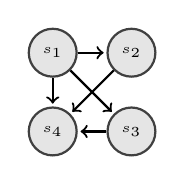
\begin{tikzpicture}[shorten >=1pt,->,scale=0.5]  
        \tikzstyle{sentence}=[circle,thick,draw=black!75,fill=black!10,minimum size=2mm]
        \tikzstyle{edge}=[draw, thick]
       \begin{scope}
         \node [sentence] (s1) at (0,2) {\tiny{$s_1$}};
         \node [sentence] (s2) at (2,2) {\tiny{$s_2$}};
         \node [sentence] (s3) at (2,0) {\tiny{$s_3$}};
         \node [sentence] (s4) at (0,0) {\tiny{$s_4$}};  
         \path[edge] (s1) edge [above] node[font=\tiny] {} (s2);
         \path[edge] (s1) edge [above] node[font=\tiny] {} (s3);
         \path[edge] (s1) edge [above] node[font=\tiny] {} (s4);
         \path[edge] (s2) edge [above] node[font=\tiny] {} (s4);
         \path[edge] (s3) edge [above] node[font=\tiny] {} (s4);

        \end{scope}        
      \end{tikzpicture}
&
%%%%%%%%%%%%%%%%%%%%%%%%%%%%%% sg 7 =126 %%%%%%%%%%%%%%%%%%%%%%%%%%%%%%
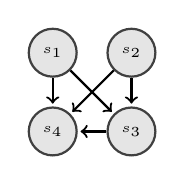
\begin{tikzpicture}[shorten >=1pt,->,scale=0.5]  
        \tikzstyle{sentence}=[circle,thick,draw=black!75,fill=black!10,minimum size=2mm]
        \tikzstyle{edge}=[draw, thick]
       \begin{scope}
         \node [sentence] (s1) at (0,2) {\tiny{$s_1$}};
         \node [sentence] (s2) at (2,2) {\tiny{$s_2$}};
         \node [sentence] (s3) at (2,0) {\tiny{$s_3$}};
         \node [sentence] (s4) at (0,0) {\tiny{$s_4$}};  
         \path[edge] (s1) edge [above] node[font=\tiny] {} (s3);
         \path[edge] (s1) edge [above] node[font=\tiny] {} (s4);
         \path[edge] (s2) edge [above] node[font=\tiny] {} (s3);
         \path[edge] (s2) edge [above] node[font=\tiny] {} (s4);
         \path[edge] (s3) edge [above] node[font=\tiny] {} (s4);
        \end{scope}        
      \end{tikzpicture}
&
%%%%%%%%%%%%%%%%%%%%%%%%%%%%%% sg 8 = 127 %%%%%%%%%%%%%%%%%%%%%%%%%%%%%%
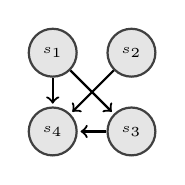
\begin{tikzpicture}[shorten >=1pt,->,scale=0.5]  
        \tikzstyle{sentence}=[circle,thick,draw=black!75,fill=black!10,minimum size=2mm]
        \tikzstyle{edge}=[draw, thick]
       \begin{scope}
         \node [sentence] (s1) at (0,2) {\tiny{$s_1$}};
         \node [sentence] (s2) at (2,2) {\tiny{$s_2$}};
         \node [sentence] (s3) at (2,0) {\tiny{$s_3$}};
         \node [sentence] (s4) at (0,0) {\tiny{$s_4$}};  
         \path[edge] (s1) edge [above] node[font=\tiny] {} (s3);
         \path[edge] (s1) edge [above] node[font=\tiny] {} (s4);
         \path[edge] (s2) edge [above] node[font=\tiny] {} (s4);
         \path[edge] (s3) edge [above] node[font=\tiny] {} (s4);
        \end{scope}        
      \end{tikzpicture}
\\
\scriptsize{$sg_9$} & \scriptsize{$sg_{10}$} & \scriptsize{$sg_{11}$} & \scriptsize{$sg_{12}$}
\\


%%%%%%%%%%%%%%%%%%%%%%%%%%%%%% sg 9 =145 %%%%%%%%%%%%%%%%%%%%%%%%%%%%%%
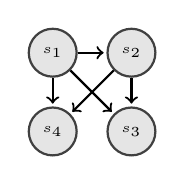
\begin{tikzpicture}[shorten >=1pt,->,scale=0.5]  
        \tikzstyle{sentence}=[circle,thick,draw=black!75,fill=black!10,minimum size=2mm]
        \tikzstyle{edge}=[draw, thick]
       \begin{scope}
         \node [sentence] (s1) at (0,2) {\tiny{$s_1$}};
         \node [sentence] (s2) at (2,2) {\tiny{$s_2$}};
         \node [sentence] (s3) at (2,0) {\tiny{$s_3$}};
         \node [sentence] (s4) at (0,0) {\tiny{$s_4$}};  
         \path[edge] (s1) edge [above] node[font=\tiny] {} (s2);
         \path[edge] (s1) edge [above] node[font=\tiny] {} (s3);
         \path[edge] (s1) edge [above] node[font=\tiny] {} (s4);
         \path[edge] (s2) edge [above] node[font=\tiny] {} (s3);
         \path[edge] (s2) edge [above] node[font=\tiny] {} (s4);
        \end{scope}        
      \end{tikzpicture}
&
%%%%%%%%%%%%%%%%%%%%%%%%%%%%%% sg 10  = 146 %%%%%%%%%%%%%%%%%%%%%%%%%%%%%%
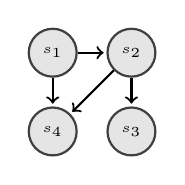
\begin{tikzpicture}[shorten >=1pt,->,scale=0.5]  
        \tikzstyle{sentence}=[circle,thick,draw=black!75,fill=black!10,minimum size=2mm]
        \tikzstyle{edge}=[draw, thick]
       \begin{scope}
         \node [sentence] (s1) at (0,2) {\tiny{$s_1$}};
         \node [sentence] (s2) at (2,2) {\tiny{$s_2$}};
         \node [sentence] (s3) at (2,0) {\tiny{$s_3$}};
         \node [sentence] (s4) at (0,0) {\tiny{$s_4$}};  
         \path[edge] (s1) edge [above] node[font=\tiny] {} (s2);
         \path[edge] (s1) edge [above] node[font=\tiny] {} (s4);
         \path[edge] (s2) edge [above] node[font=\tiny] {} (s3);
         \path[edge] (s2) edge [above] node[font=\tiny] {} (s4);
        \end{scope}        
      \end{tikzpicture}
&
%%%%%%%%%%%%%%%%%%%%%%%%%%%%%% sg 11  = 156 %%%%%%%%%%%%%%%%%%%%%%%%%%%%%%
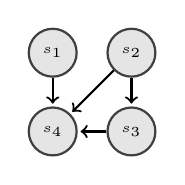
\begin{tikzpicture}[shorten >=1pt,->,scale=0.5]  
        \tikzstyle{sentence}=[circle,thick,draw=black!75,fill=black!10,minimum size=2mm]
        \tikzstyle{edge}=[draw, thick]
       \begin{scope}
         \node [sentence] (s1) at (0,2) {\tiny{$s_1$}};
         \node [sentence] (s2) at (2,2) {\tiny{$s_2$}};
         \node [sentence] (s3) at (2,0) {\tiny{$s_3$}};
         \node [sentence] (s4) at (0,0) {\tiny{$s_4$}};  
         \path[edge] (s1) edge [above] node[font=\tiny] {} (s4);
         \path[edge] (s2) edge [above] node[font=\tiny] {} (s3);
         \path[edge] (s2) edge [above] node[font=\tiny] {} (s4);
         \path[edge] (s3) edge [above] node[font=\tiny] {} (s4);
        \end{scope}        
      \end{tikzpicture}
&
%%%%%%%%%%%%%%%%%%%%%%%%%%%%%% sg 12 = 165 %%%%%%%%%%%%%%%%%%%%%%%%%%%%%%
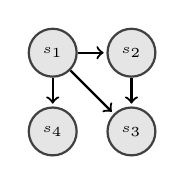
\begin{tikzpicture}[shorten >=1pt,->,scale=0.5]  
        \tikzstyle{sentence}=[circle,thick,draw=black!75,fill=black!10,minimum size=2mm]
        \tikzstyle{edge}=[draw, thick]
       \begin{scope}
         \node [sentence] (s1) at (0,2) {\tiny{$s_1$}};
         \node [sentence] (s2) at (2,2) {\tiny{$s_2$}};
         \node [sentence] (s3) at (2,0) {\tiny{$s_3$}};
         \node [sentence] (s4) at (0,0) {\tiny{$s_4$}};  
         \path[edge] (s1) edge [above] node[font=\tiny] {} (s2);
         \path[edge] (s1) edge [above] node[font=\tiny] {} (s3);
         \path[edge] (s1) edge [above] node[font=\tiny] {} (s4);
         \path[edge] (s2) edge [above] node[font=\tiny] {} (s3);
        \end{scope}        
      \end{tikzpicture}
\\
\scriptsize{$sg_{13}$} & \scriptsize{$sg_{14}$} & \scriptsize{$sg_{15}$} & \scriptsize{$sg_{16}$}
\\

%%%%%%%%%%%%%%%%%%%%%%%%%%%%%% sg 13 = 172 %%%%%%%%%%%%%%%%%%%%%%%%%%%%%%
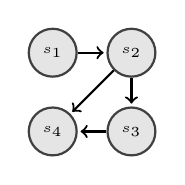
\begin{tikzpicture}[shorten >=1pt,->,scale=0.5]  
        \tikzstyle{sentence}=[circle,thick,draw=black!75,fill=black!10,minimum size=2mm]
        \tikzstyle{edge}=[draw, thick]
       \begin{scope}
         \node [sentence] (s1) at (0,2) {\tiny{$s_1$}};
         \node [sentence] (s2) at (2,2) {\tiny{$s_2$}};
         \node [sentence] (s3) at (2,0) {\tiny{$s_3$}};
         \node [sentence] (s4) at (0,0) {\tiny{$s_4$}};  
         \path[edge] (s1) edge [above] node[font=\tiny] {} (s2);
         \path[edge] (s2) edge [above] node[font=\tiny] {} (s3);
         \path[edge] (s2) edge [above] node[font=\tiny] {} (s4);
         \path[edge] (s3) edge [above] node[font=\tiny] {} (s4);
        \end{scope}        
      \end{tikzpicture}
&
%%%%%%%%%%%%%%%%%%%%%%%%%%%%%% sg 14 =192 %%%%%%%%%%%%%%%%%%%%%%%%%%%%%%
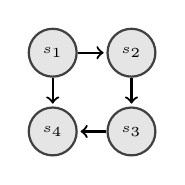
\begin{tikzpicture}[shorten >=1pt,->,scale=0.5]  
        \tikzstyle{sentence}=[circle,thick,draw=black!75,fill=black!10,minimum size=2mm]
        \tikzstyle{edge}=[draw, thick]
       \begin{scope}
         \node [sentence] (s1) at (0,2) {\tiny{$s_1$}};
         \node [sentence] (s2) at (2,2) {\tiny{$s_2$}};
         \node [sentence] (s3) at (2,0) {\tiny{$s_3$}};
         \node [sentence] (s4) at (0,0) {\tiny{$s_4$}};  
         \path[edge] (s1) edge [above] node[font=\tiny] {} (s2);
         \path[edge] (s1) edge [above] node[font=\tiny] {} (s4);
         \path[edge] (s2) edge [above] node[font=\tiny] {} (s3);
         \path[edge] (s3) edge [above] node[font=\tiny] {} (s4);
        \end{scope}        
      \end{tikzpicture}
&
%%%%%%%%%%%%%%%%%%%%%%%%%%%%%% sg 15 =193 %%%%%%%%%%%%%%%%%%%%%%%%%%%%%%
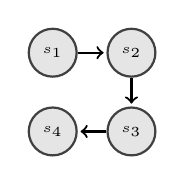
\begin{tikzpicture}[shorten >=1pt,->,scale=0.5]  
        \tikzstyle{sentence}=[circle,thick,draw=black!75,fill=black!10,minimum size=2mm]
        \tikzstyle{edge}=[draw, thick]
       \begin{scope}
         \node [sentence] (s1) at (0,2) {\tiny{$s_1$}};
         \node [sentence] (s2) at (2,2) {\tiny{$s_2$}};
         \node [sentence] (s3) at (2,0) {\tiny{$s_3$}};
         \node [sentence] (s4) at (0,0) {\tiny{$s_4$}};  
         \path[edge] (s1) edge [above] node[font=\tiny] {} (s2);
         \path[edge] (s2) edge [above] node[font=\tiny] {} (s3);
         \path[edge] (s3) edge [above] node[font=\tiny] {} (s4);
        \end{scope}        
      \end{tikzpicture}
&
%%%%%%%%%%%%%%%%%%%%%%%%%%%%%% sg 16 = 216 %%%%%%%%%%%%%%%%%%%%%%%%%%%%%%
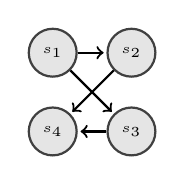
\begin{tikzpicture}[shorten >=1pt,->,scale=0.5]  
        \tikzstyle{sentence}=[circle,thick,draw=black!75,fill=black!10,minimum size=2mm]
        \tikzstyle{edge}=[draw, thick]
       \begin{scope}
         \node [sentence] (s1) at (0,2) {\tiny{$s_1$}};
         \node [sentence] (s2) at (2,2) {\tiny{$s_2$}};
         \node [sentence] (s3) at (2,0) {\tiny{$s_3$}};
         \node [sentence] (s4) at (0,0) {\tiny{$s_4$}};  
         \path[edge] (s1) edge [above] node[font=\tiny] {} (s2);
         \path[edge] (s1) edge [above] node[font=\tiny] {} (s3);
         \path[edge] (s2) edge [above] node[font=\tiny] {} (s4);
         \path[edge] (s3) edge [above] node[font=\tiny] {} (s4);
        \end{scope}        
      \end{tikzpicture}
\\
\scriptsize{$sg_{17}$} & \scriptsize{$sg_{18}$} & \scriptsize{$sg_{19}$} & \scriptsize{$sg_{20}$}
\\

%%%%%%%%%%%%%%%%%%%%%%%%%%%%%% sg 17 = 217 %%%%%%%%%%%%%%%%%%%%%%%%%%%%%%
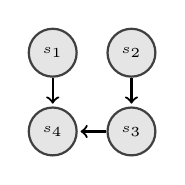
\begin{tikzpicture}[shorten >=1pt,->,scale=0.5]  
        \tikzstyle{sentence}=[circle,thick,draw=black!75,fill=black!10,minimum size=2mm]
        \tikzstyle{edge}=[draw, thick]
       \begin{scope}
         \node [sentence] (s1) at (0,2) {\tiny{$s_1$}};
         \node [sentence] (s2) at (2,2) {\tiny{$s_2$}};
         \node [sentence] (s3) at (2,0) {\tiny{$s_3$}};
         \node [sentence] (s4) at (0,0) {\tiny{$s_4$}};  
         \path[edge] (s1) edge [above] node[font=\tiny] {} (s4);
         \path[edge] (s2) edge [above] node[font=\tiny] {} (s3);
         \path[edge] (s3) edge [above] node[font=\tiny] {} (s4);
        \end{scope}        
      \end{tikzpicture}

&
%%%%%%%%%%%%%%%%%%%%%%%%%%%%%% sg 18 = 227 %%%%%%%%%%%%%%%%%%%%%%%%%%%%%%
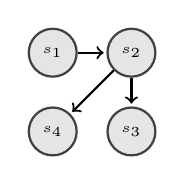
\begin{tikzpicture}[shorten >=1pt,->,scale=0.5]  
        \tikzstyle{sentence}=[circle,thick,draw=black!75,fill=black!10,minimum size=2mm]
        \tikzstyle{edge}=[draw, thick]
       \begin{scope}
         \node [sentence] (s1) at (0,2) {\tiny{$s_1$}};
         \node [sentence] (s2) at (2,2) {\tiny{$s_2$}};
         \node [sentence] (s3) at (2,0) {\tiny{$s_3$}};
         \node [sentence] (s4) at (0,0) {\tiny{$s_4$}};  
         \path[edge] (s1) edge [above] node[font=\tiny] {} (s2);
         \path[edge] (s2) edge [above] node[font=\tiny] {} (s3);
         \path[edge] (s2) edge [above] node[font=\tiny] {} (s4);
        \end{scope}        
      \end{tikzpicture}

&
%%%%%%%%%%%%%%%%%%%%%%%%%%%%%% sg 19 =237 %%%%%%%%%%%%%%%%%%%%%%%%%%%%%%
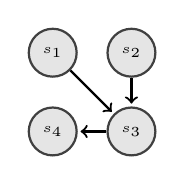
\begin{tikzpicture}[shorten >=1pt,->,scale=0.5]  
        \tikzstyle{sentence}=[circle,thick,draw=black!75,fill=black!10,minimum size=2mm]
        \tikzstyle{edge}=[draw, thick]
       \begin{scope}
         \node [sentence] (s1) at (0,2) {\tiny{$s_1$}};
         \node [sentence] (s2) at (2,2) {\tiny{$s_2$}};
         \node [sentence] (s3) at (2,0) {\tiny{$s_3$}};
         \node [sentence] (s4) at (0,0) {\tiny{$s_4$}};  
         \path[edge] (s1) edge [above] node[font=\tiny] {} (s3);
         \path[edge] (s2) edge [above] node[font=\tiny] {} (s3);
         \path[edge] (s3) edge [above] node[font=\tiny] {} (s4);
        \end{scope}        
      \end{tikzpicture}
&
%%%%%%%%%%%%%%%%%%%%%%%%%%%%%% sg 20 =246 %%%%%%%%%%%%%%%%%%%%%%%%%%%%%%
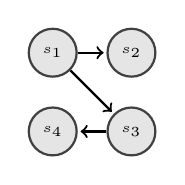
\begin{tikzpicture}[shorten >=1pt,->,scale=0.5]  
        \tikzstyle{sentence}=[circle,thick,draw=black!75,fill=black!10,minimum size=2mm]
        \tikzstyle{edge}=[draw, thick]
       \begin{scope}
         \node [sentence] (s1) at (0,2) {\tiny{$s_1$}};
         \node [sentence] (s2) at (2,2) {\tiny{$s_2$}};
         \node [sentence] (s3) at (2,0) {\tiny{$s_3$}};
         \node [sentence] (s4) at (0,0) {\tiny{$s_4$}};  
         \path[edge] (s1) edge [above] node[font=\tiny] {} (s3);
         \path[edge] (s1) edge [above] node[font=\tiny] {} (s2);
         \path[edge] (s3) edge [above] node[font=\tiny] {} (s4);
        \end{scope}        
      \end{tikzpicture}
\\
\scriptsize{$sg_{21}$} & \scriptsize{$sg_{22}$} & \scriptsize{$sg_{23}$} & \scriptsize{$sg_{24}$}
\\

%%%%%%%%%%%%%%%%%%%%%%%%%%%%%% sg 21 =277 %%%%%%%%%%%%%%%%%%%%%%%%%%%%%%
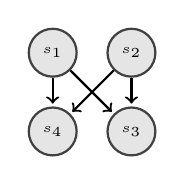
\begin{tikzpicture}[shorten >=1pt,->,scale=0.5]  
        \tikzstyle{sentence}=[circle,thick,draw=black!75,fill=black!10,minimum size=2mm]
        \tikzstyle{edge}=[draw, thick]
       \begin{scope}
         \node [sentence] (s1) at (0,2) {\tiny{$s_1$}};
         \node [sentence] (s2) at (2,2) {\tiny{$s_2$}};
         \node [sentence] (s3) at (2,0) {\tiny{$s_3$}};
         \node [sentence] (s4) at (0,0) {\tiny{$s_4$}};  
         \path[edge] (s1) edge [above] node[font=\tiny] {} (s3);
         \path[edge] (s1) edge [above] node[font=\tiny] {} (s4);
         \path[edge] (s2) edge [above] node[font=\tiny] {} (s3);
         \path[edge] (s2) edge [above] node[font=\tiny] {} (s4);
        \end{scope}        
      \end{tikzpicture}
&
%%%%%%%%%%%%%%%%%%%%%%%%%%%%%% sg 22 =278 %%%%%%%%%%%%%%%%%%%%%%%%%%%%%%
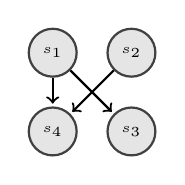
\begin{tikzpicture}[shorten >=1pt,->,scale=0.5]  
        \tikzstyle{sentence}=[circle,thick,draw=black!75,fill=black!10,minimum size=2mm]
        \tikzstyle{edge}=[draw, thick]
       \begin{scope}
         \node [sentence] (s1) at (0,2) {\tiny{$s_1$}};
         \node [sentence] (s2) at (2,2) {\tiny{$s_2$}};
         \node [sentence] (s3) at (2,0) {\tiny{$s_3$}};
         \node [sentence] (s4) at (0,0) {\tiny{$s_4$}};  
         \path[edge] (s1) edge [above] node[font=\tiny] {} (s3);
         \path[edge] (s1) edge [above] node[font=\tiny] {} (s4);
         \path[edge] (s2) edge [above] node[font=\tiny] {} (s4);
        \end{scope}        
      \end{tikzpicture}

&
%%%%%%%%%%%%%%%%%%%%%%%%%%%%%% sg 23 = 289  %%%%%%%%%%%%%%%%%%%%%%%%%%%%%%
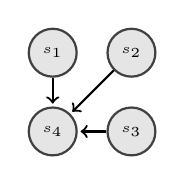
\begin{tikzpicture}[shorten >=1pt,->,scale=0.5]  
        \tikzstyle{sentence}=[circle,thick,draw=black!75,fill=black!10,minimum size=2mm]
        \tikzstyle{edge}=[draw, thick]
       \begin{scope}
         \node [sentence] (s1) at (0,2) {\tiny{$s_1$}};
         \node [sentence] (s2) at (2,2) {\tiny{$s_2$}};
         \node [sentence] (s3) at (2,0) {\tiny{$s_3$}};
         \node [sentence] (s4) at (0,0) {\tiny{$s_4$}};  
         \path[edge] (s1) edge [above] node[font=\tiny] {} (s4);
         \path[edge] (s2) edge [above] node[font=\tiny] {} (s4);
         \path[edge] (s3) edge [above] node[font=\tiny] {} (s4);
        \end{scope}        
      \end{tikzpicture}

&
%%%%%%%%%%%%%%%%%%%%%%%%%%%%%% sg 24 = 304 %%%%%%%%%%%%%%%%%%%%%%%%%%%%%%
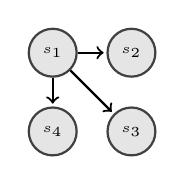
\begin{tikzpicture}[shorten >=1pt,->,scale=0.5]  
        \tikzstyle{sentence}=[circle,thick,draw=black!75,fill=black!10,minimum size=2mm]
        \tikzstyle{edge}=[draw, thick]
       \begin{scope}
         \node [sentence] (s1) at (0,2) {\tiny{$s_1$}};
         \node [sentence] (s2) at (2,2) {\tiny{$s_2$}};
         \node [sentence] (s3) at (2,0) {\tiny{$s_3$}};
         \node [sentence] (s4) at (0,0) {\tiny{$s_4$}};  
         \path[edge] (s1) edge [above] node[font=\tiny] {} (s2);
         \path[edge] (s1) edge [above] node[font=\tiny] {} (s3);
         \path[edge] (s1) edge [above] node[font=\tiny] {} (s4);
        \end{scope}        
      \end{tikzpicture}
\end{tabular}
\caption{Frequent subgraphs with four nodes where $t<u<v<w$.}\label{4node_subgraphs}
\end{figure}


\paragraph{Results.}
%
We use the Pearson correlation coefficient to find features correlated with readability scores. 
It takes feature values and readability scores of all documents and returns $-1\leq\rho\leq+1$. 
A high value of $|\rho|$ shows a strong correlation. 
We report statistical significance on the $0.05$-level. 
\newcite{pitler08} also showed that each entity transition feature extracted from the entity grid representation \cite{barzilay08} of document individually does not significantly correlate with human readability ratings. 
Therefore, we report the correlation of our coherence models encoded in graph features and compare them with the average outdegree metric used in the entity graph  model as the state-of-the-art coherence model \cite{}.

\begin{table}[!t]
\centering
\begin{tabular}{lrc}
\hline
 & $\rho$ & p\_value\\\hline
 $P_u$ & $-0.013$ & $0.949$ \\
 $P_w$ & $0.151$  & $0.452$\\
 $P_{acc}$ & $0.150$ & $0.455$\\
\hline
\end{tabular}
\caption{The correlation of the average outdegree of different graphs with human readability ratings.}
 \label{table:OD_pearson}
\end{table}

Table \ref{table:OD_pearson} shows the correlation of the average outdegree feature of three types of projection graphs defined in the entity graph model. 
The first interpretation of results is that the average outdegree of none of the projection graphs are significantly correlated with rankings assigned by humans. 
However, the average outdegree of $P_w^{ER}$ is highly correlated with human readability ratings that is compatible with the readability results reported on the Encyclopedia Britannica dataset in the previous chapter. 



\begin{table}[!h]
\centering
\begin{small}
\begin{tabular}{lrc}
\hline
   & $\rho$ & p\_value\\\hline
\textbf{Number of Components} & $\mathbf{-0.391}$ & $\mathbf{0.044}$  \\\hline

\multicolumn{3}{l}{\textbf{Frequency of 3-node Patterns}} \\
 $sg_1$ &  $0.310$ & $0.116$\\
 $sg_2$ & $-0.325$ & $0.098$\\
$\mathbf{sg_3}$ & $\mathbf{-0.384}$ & $\mathbf{0.048}$\\
 $sg_4$ &  $0.108$ & $0.592$\\\hline
\end{tabular}
\end{small}
\caption{The frequency of pattern $sg_3$ is significantly negatively correlated to readability.}
 \label{table:3node_pearson}
\end{table}

Table \ref{table:3node_pearson} shows the Pearson correlation coefficient and their corresponding p\_value between frequency of coherence patterns and readability scores assigned by humans. 
Pattern $sg_3$ is significantly and negatively correlated with human readability rankings;  confirming this intuition that documents with many shifts in focus of attention are perceived more difficult to read. 

We notice that the frequency of pattern $sg_1$ is positively correlated with readability rankings, not significantly though. 
This pattern captures a sentence that represents some information, that is limited in our model to entities, then  subsequent sentences are about those information. 
Our results show that the easier to read documents contains many of this pattern because this pattern positively correlated with human rankings. 
The frequency of pattern $sg_2$ is negatively correlated with human rankings, showing that this pattern has not been observed in coherent documents as frequent as in incoherent documents. 
This matches with this linguistic phenomena saying that  processing sentences that are independent and then are connected in a subsequent sentence is difficult and ambiguous for readers. 
Interestingly, the structural difference between pattern $sg_2$ and pattern $sg_1$ can be interpreted as the order of sentences. 
If sentence $s_t$ was before $s_u$ in pattern $sg_2$, then the pattern would look like $sg_1$ that is a property of coherent texts. 
This means that these patterns can capture the order of information presented in sentences as well. 

% The number of components has a strong and significant negative correlation with human readability ratings\footnote{This supports
% \newcite{karamanis09} who report that NOCB transitions in the centering model can be used for the sentence ordering task.}, suggesting that simple properties of graphs measure text
% coherence. 
 



\begin{table}[!t]
\centering
\begin{small}
\begin{tabular}{lcrc}
\hline
   & number of edges & $\rho$ & p\_value\\\hline
$sg_1$ & 6 & 0.103 & 0.609   \\
$sg_2$ & 5 & $-0.212$ & 0.288    \\
$sg_3$  & 5 &   $-0.176$ & 0.380      \\
$sg_4$  & 4 &$-0.257$ & 0.196    \\
$sg_5$ & 5 &$-0.140$ & 0. 486   \\
$sg_6$  & 5 &   0.200 &  0.317  \\
$\mathbf{sg_7}$ & \textbf{5} & $\mathbf{-0.402}$ & \textbf{0.038}  \\
$sg_8$  & 4 &$-0.317$ & 0.107 \\
$sg_9$ & 5 & 0.153 & 0.446   \\
$sg_{10}$ & 4 & $-0.238$ & 0.232    \\
$\mathbf{sg_{11}}$ & \textbf{4} & $\mathbf{-0.509}$     & \textbf{0.007}\\
$\mathbf{sg_{12}}$  & \textbf{4} &\textbf{0.449} & \textbf{0.019}    \\
$sg_{13}$  & 4 & $-0.045$ & 0.824    \\
$sg_{14}$ & 4 & $-0.033$ & 0.870\\
$sg_{15}$ & 3 &$-0.358$ & 0.067    \\
$sg_{16}$ &     4 &$-0.068$ & 0.736    \\
$sg_{17}$  & 3 & $-0.308$ & 0.118    \\
$\mathbf{sg_{18}}$ & \textbf{3} & $\mathbf{-0.546}$      & \textbf{0.003}   \\
$\mathbf{sg_{19}}$ & \textbf{3} & $\mathbf{-0.601}$ & \textbf{0.001}   \\
$sg_{20}$ & 3 & 0.094   & 0.641 \\
$sg_{21}$  & 4 & 0.068 & 0.736   \\
$sg_{22}$ &  3& $-0.374$ &  0.055  \\
$sg_{23}$ &     3&$-0.314$ & 0.111 \\
$sg_{24}$ &     3& 0.100 & 0.620  \\
\hline
\end{tabular}
\end{small}
\caption{The correlation between the frequency of 4-node patterns and readability ratings.}\label{table:correlation_4node_subgraph}
\end{table}


Table \ref{table:correlation_4node_subgraph} shows the Pearson correlation coefficient between the frequency of 4-node patterns and readability ratings assigned by humans.  
First, most patterns with less than four edges are negatively correlated with readability rankings, except $sg_{20}$ and $sg_{24}$ which are weakly correlated with readability. 
Few connections between sentences make the text difficult to read.

Among all patterns that have a positive correlation coefficient with human rankings, 
$sg_{12}$ has the highest correlation coefficient.  
In contrast, the most negatively correlation efficient is for pattern $sg_{11}$. 
When we compare these two patterns, these two patterns have the same number of edges but  different style of connectivity.
This confirms our hypotheses: (i) The connectivity structure of projection graphs of coherent texts are similar to each other and different with those of incoherent texts. 
(ii) The frequency of subgraphs can encode the connectivity structure of projection graphs and consequently coherence. 
\newcite[p.29]{stoddard91} explains this by the \emph{ambiguity node}\ phenomenon: ``[...] in some cases, there may be more
than one logical, possible node for a given cohesive element in a text, in which case, a reader may see the resulting ambiguity but not be able to decide between the choices''. 
E.g., in $sg_{11}$ a reader may make a decision about the focus of attention in $s_w$, while in $sg_{12}$ the focus of attention of $s_w$ is the same as the
focus of attention of $s_t$. 
This phenomenon can also be observed in all positively correlated subgraphs. 
If readers have to return to one point in the text, they prefer to return to a sentence which is the core of the preceding sentences.
Finally, we conclude that in all strongly negative correlated patterns, a subgraph suffers either from edge shortage or the \textit{ambiguity node}\ phenomenon like $sg_7$.


Considering the correlation of 3-node subgraphs in Table \ref{table:3node_pearson} and 4-node subgraphs in Table \ref{table:correlation_4node_subgraph}, two results are noticeable.
First, there are more strongly correlated 4-node patterns than 3-node pattens, confirming our hypothesis that larger subgraphs capture more information about the connectivity style of projection graphs and therefore more powerful predictor of coherence.  
Second, the Pearson correlation coefficient obtained for $sg_{12}$ in 4-node subgraphs is greater than the one of than $sg_4$ in 3-node subgraphs, this can be because $sg_{12}$ captures more circumstances about connectivity of $s_t$. 
However, we should refrain of interpreting too much into these patterns.


Following observations conclude the results of this experiment:

\begin{itemize}
	\item The average outdegree metric is not significantly correlated with human rankings assigned to documents in the examined dataset 

	\item The connectivity style of projection graphs representing entity-based relations among sentences of coherent texts are similar to each other and different with those of incoherent texts

	\item The connectivity style of a projection graph can be encoded by the frequency of coherence patterns 

	\item We found our coherence patterns that mined automatically from projection graphs are roughly similar to patterns introduced by \newcite{danes74}

	\item Our coherence patterns are not limited to adjacent sentences and they can model long distant connections as well 

\end{itemize}


\subsection{Readability Ranking} 
\label{subsec:Readability Ranking}
%
The readability of a document depends on various factors ranging from the length of words and sentences that are used in the document to more complex factors such as the familiarity of vocabularies for a reader and semantic relations among sentences. 
Although coherence is one of the crucial factors of easy to read texts but it is not sufficient to predict the readability score of documents. 
Instead, coherence models can be evaluated by ranking documents. 
Given that easier to read documents are more coherent than difficult documents, we can rank documents with respect to their readability. 
Then, we investigate how well a ranking of documents based on their coherence match with the ranking based on readability. 
A coherence model that ranks documents more similar to rankings based on readability is a better coherence model for the readability task. 

In addition, the readability ranking task may in fact be the more natural one, since in most applications the main concern is with the relative quality of documents rather than their absolute scores. 


\paragraph{Implementation Details. }
%
We follow \newcite{pitler08} and rank documents in a pairwise approach with respect to their readability. 
Text pairs include texts of the dataset (introduced in Section \ref{}) that their readability scores differ by at least $0.5$. 
This criteria ensures that the difference in readability ratings of texts in a text pair is noticeable enough that a coherence model distinguishes their difference. 

We treat this as a classification problem such that given a text pair, is the first document in the pair easier to read than the second one? 
We employ WEKA's linear support vector implementation (SMO)  to classify the pairs.
The SMO model is supplied by different sets of coherence features representing the coherence of each text. 

The first set of coherence features is grammatical transitions of entities proposed by the entity grid model. 
All nouns in texts are taken as mentions of entities in a text. 
The gold parse trees from the Penn Treebank \cite{marcus94} are employed to extract all nouns in a document. 
We use Stanford CoreNLP\footnote{http://nlp.stanford. edu/software/corenlp.shtml} to extract stems of all nouns and then nouns with identical stem make entities. 
\textbf{[TO DO: do you use coherencetoolkit to extract entity grids? or did you implement it yourself? How do you extract grammatical roles of entities? Stanford dependency parser or BrownCoherenceToolkit?]}

The performance of a set of coherence features for the readability ranking task is measured by the accuracy of rankings  predicted by the SMO model when it is supplied by the feature set. 
The accuracy is calculated as follows:

\begin{equation}
Accuracy = \frac{\textit{number of correct rankings}}{\textit{number of pairs}}. 
\end{equation}

Since the dataset is not accompanied by any standard split of training and test sets, we use 10-fold cross-validation for comparing the quality of different coherence feature sets. 
The reported accuracy is the average over all accuracies obtained from all runs of 10-fold cross-validation. 

\textbf{[What is the number pairs?]}

\paragraph{Results. }
%
Table \ref{table:classification_task} summarizes the results of the readability ranking task. 

We compare our graph-based coherence features obtained from the k-node subgraphs of projection graphs with the proposed features obtained from grammatical transitions of entities by the entity gird model. 
In order to compare different sets of coherence features, we employ the same machine learning model, (i.e. SMO) for training and testing on each feature set. 
Therefore in Table \ref{table:classification_task},  we only show the name of feature set that is used to represent the coherence property of texts, all other settings are unique. 

In Table \ref{table:classification_task}, Baseline features are the frequency of grammatical transitions of entities over sentences. 
This feature set is also evaluated\footnote{The accuracy reported in their paper is $79.42\%$. Our reimplementation achieves higher accuracy, because our dataset has three articles less.} as coherence features on this dataset by \newcite{pitler08}.

\begin{table}[!h]
\centering
\begin{small}
\begin{tabular}{@{}lc@{}}
\hline
\textbf{Features} & \textbf{Accuracy} \\\hline
\multicolumn{2}{l}{\textbf{Baselines}} \\
None (Majority class) & 47.85\% \\
Baseline features \cite{pitler08} & 83.25\% \\\hline
\multicolumn{2}{l}{\textbf{Graph-based Features}} \\
%Number of components & 61.72\%\\
3-node & 79.43\% \\
4-node & 89.00\%  \\
3-node \& 4-node & 88.52\% \\
Baseline + 4-node & 93.30\% \\
\hline
\end{tabular}
\end{small}
\caption{SVM prediction accuracy.}
\label{table:classification_task}
\end{table}

When classifying with the frequency of 3-node subgraphs as coherence features, the obtained accuracy is lower than when the baseline coherence features are employed.  
This could have two reasons. 
The entity grid features represent grammatical role transitions of entities, that is more informative than the connections used in 3-node subgraphs only model the occurrence of entities between sentences. 
On the other hand, 3-node patterns are small and more likely to occur in most projection graphs, so their frequencies cannot distinguish between coherent and incoherent texts easily. 

The feature set containing the frequency of 4-node patterns outperforms the baseline feature set by about $6\%$. 
This confirms our hypothesis that the entity-based connectivity structure among sentences, which is modeled by projection graphs, distinguishes coherent texts from incoherent texts. 
An advantage of 4-node subgraphs over the baseline features is that long-distant relations are also taken into account. 
On the other hand, our coherence patterns lack the grammatical grammatical of entities. 
Our other hypothesis was that since 4-node patterns are larger than 3-node patterns, they have more capacity, in terms of nodes and edges, to model the connectivity of nodes in projection graphs and therefore coherence. 
This hypothesis is confirmed by comparing the accuracy of 4-node subgraphs against 3-node subgraphs.
4-node subgraphs outperforms 3-node subgraphs by $10\%$ difference in accuracy . 
That is a considerable improvement that verifies that larger subgraphs capture connectivity style between nodes of projection graphs much better.   

In another experiment, we use the frequency of all 3-node and 4-node subgraphs in projection graphs. 
The obtained accuracy is better than the one with only 3-node patters but slightly worse  ($-1\%$) than the one with only 4-node patterns. 
An explanation for this is that 4-node subgraph implicitly contain 3-node subgraphs in themselves. 
Combining these two sets of features does not probably provide any useful information for modeling the connectivity style of projection graphs more than what exists in 4-node subgraphs. 

Finally, the combination of baseline coherence features, (i.e. the frequency of grammatical transitions of entities over adjacent sentences), and 4-node subgraphs achieves the best accuracy. 
This might be interpreted in this way that although our coherence patterns capture the connectivity structure among sentences of a text, integrating linguistic information such syntactic transitions of entities may improve the quality of a coherence model.  



%This idea that each word in a text will be considered a cohesive ties is introduced in \newcite{stoddard91}. 
% \newcite{stoddard91} in her analysis expresses that designing a research package for analyzing of  cohesion patterns is complicated because of different number of cohesive ties, the number of evaluated written texts by human readers. 
% The narrowing can be done in any one or several ways. 
% One is the selection of the type of cohesion ties to be analyzed. 
% The second is the selection of the corpus. 
% Following our entity-based setting in previous chapters, we limit our cohesive ties are restricted version of references in \newcite{halliday76}, the string match between nouns. 
% If, however, a writer chooses to simply repeat nodes without using many cohesive elements, we might expect that readers would find  the content equally cohesive (but probably boring for its repetitiveness).
% There would be a relationship between the phenomenon of node repetition and memory retention \cite{stoddard91}. 
%Certainly, cohesive ties that span sentence and paragraph boundaries have greater potential for unifying a text and making it more cohesive. 

\subsection{Automatic Summarization}
\label{subsec:automatic_summarization}
%
Automatic summarization has been receiving a lot of attentions by researchers in natural language processing because of its potential for various information access applications. 
For instance it is useful for tools that aid users navigate and digest web content (e.g., news, social media, product reviews), question answering, and personalized recommendation engines. 
Single document summarization is the task of producing a shorter version of a document while preserving its information content. 
This task is perhaps the most basic of summarization tasks that have been identified over the years \cite{nenkova11}. 

A basic approach to single document summarization is extractive in that a summary is produced by identifying and concatenating the most important sentences in a document. 
Ideally, information in selected sentences for a summary should be most important information of a document; have enough variance (or minimum redundancy); and be presented in a coherent way in the summary to be readable. 

Developing an extractive summarizer that jointly optimizes these three crucial factors -- importance, diversity, and coherence -- is a challenging task, because the inclusion of relevant sentences relies not only on properties of the sentences themselves, also properties of every other sentences in a summary. 
Moreover, sine the length of a summary is limited\footnote{Forcing summaries to obey a length constraint is a common set-up in summarization as it allows for a fair empirical comparison between different possible outputs. 
 Furthermore, it represents an important ``real world'' scenario where summaries are generated in order to be displayed on small screens, such as mobile devices.
} making a balance between these three factors is difficult. 
For example, a summarizer may need to select a sentence that contains less important information with respect to other sentences, just to make other selected sentences coherent. 

This optimization problem is typically solved in one of two ways:  Optimizing these factors separately; Optimizing all criteria in tandem. 
The work of \cite{mckeown99} is an example of the first solution. 
It presents a \mbox{two-stage} system in which sentences are initially clustered, and then representative sentences are chosen from each cluster to be included into the final summary. 
Here, the clustering stage minimizes redundancy and the representative sentence selection maximizes importance.
The work of \cite{carbonell98} is an example of the second solution.  
It propose a global model through the use of the maximum marginal relevance (MMR) criteria, which scores sentences under consideration as a weighted combination of importance plus redundancy with sentences already in the summary. 
Summaries are then created with an approximate greedy procedure that incrementally includes the sentence that maximizes this criteria. Greedy MMR style algorithms are still a standard baseline for summarization. 

One of the popular approaches for global optimization problems is the Integer Linear Programming (ILP) formulation. 
ILP techniques have been used to solve many intractable inference problems in NLP applications. 
Examples include applications to sentence compression \cite{clarke10,filippova13}, coreference resolution \cite{denis09},  syntactic parsing \cite{klenner07a}, as well as semantic role labeling \cite{punyakanok04b}.
\cite{marciniak05b,mcdonald07,bergkirkpatrick11,woodsend12,lichen13a,hirao13}.
In an ILP approach, an optimization problem is modeled by an objective function and some constraints. 
Solving arbitrary ILPs is an \mbox{NP-hard} problem. 
However, ILPs are a well studied optimization problem with efficient \mbox{branch-and-bound} algorithms for finding the optimal solution. 
Similar to the other NLP applications, ILP has been popularly employed for automatic summarization 
\cite{marciniak05b,mcdonald07,bergkirkpatrick11,woodsend12,lichen13a,hirao13}.  

\newcite{parveen15} propose an automatic summarizer using ILP.  
The objective of the optimization is to select a subset of sentences from an input document such that the selected sentences produce a summary that is optimal in terms of importance, non-redundancy, and coherence. 
This model is of our interest, because it sets up their optimization problem on the entity graph representations of documents. 
Given an input document, the importance and non-redundancy of selected sentences for a summary are measured by the bipartite entity graph of the input document. 
They hypothesis that the outdegree of each node in the projection graph of the input document measures how crucial the corresponding sentence with the node is crucial for coherence of the summary.  
This has two weaknesses: 

\begin{itemize}
	\item 
	The entity-graph coherence model uses the average outdegree of the projection graph of a document to measure the coherence of the entire document. 
	Limiting this metric to each sentence, in this way that nodes of projection graphs with higher outdegree represent sentences that are more crucial for coherence, biases the summarizer to select more sentences from the begging of documents. 
	This happens because projection graphs are directed to capture the sentence order of documents, so early sentences in documents are more connected to other sentences. 


	\item The outdegree of sentence nodes are computed in projection graphs of input documents for the summarization model,  
	whereas the goal is to select sentences that make the produced summary more coherent. So the connectivity of sentences should be evaluated with respect to only other selected sentences for the summary, not all sentences in the document. 


	\item 
	We have shown that the average outdegree is not the best metric for encoding the connectivity style of projection graphs and therefore coherence. 

\end{itemize} 

Here, we emphasize on the coherence aspect of the proposed summarization system by \newcite{parveen15} with two motivations:
\begin{itemize}
	\item Using the automatic summarization task as another application for evaluating our graph-based coherence patterns, introduced in Chapter \ref{}

	\item Improving the performance of the examined summarization  model by integrating our coherence patterns, rather than outdegree, into the summarization model
\end{itemize}

Our intuition is that human generated summaries given in a dataset are expected to be coherent enough to be readable.
So if a summarization system extracts sentences of a document such that their connectivity styles in the produced summary are similar to the connectivity styles of sentences in human generated summaries, then the produced summary is sufficiently well-connected and therefore coherent. 
 
% We employ discourse entities as the unit of information that relate sentences because they can also be served to measure the importance, diversity of sentences in a summary. 
% Sentences that contain prominent entities of a document are important to be extracted. 
% A summary whose sentences refer to few entities may contain redundant information. 
% The order of sentences in a summary and the way that they share entities make the summary coherent. 
% We extract useful connectivity patterns for automatic summarization using a data-driven approach. 
% Given gold summaries, we represent entity relations between sentences of each summary via a graph whose nodes are sentences and edges are entity-based relations between sentences. 
% By applying a subgraph mining method to graph representations of gold summaries all subgraphs (coherence patterns) are extracted. 
% More frequent patterns are preferred to be observed in a machine generated summary more than other patterns. 
% So the frequency of patterns in gold summaries is used as an indicator of human preferences over patterns to be used for connecting sentences in a summary. 
% These patterns and their frequency are combined with other conditions for importance and diversity of sentences using the linear programming fashion. 

% We run our summarizers on DUC dataset that is commonly used for this task, and on PubMed corpus that consists of scientific articles. 
% Summarizing texts of scientific articles are taken difficult as multi-document summarization. 
% In addition, articles in PubMed corpus are associated with some summaries written by editors of the PubMed journal that can be used for evaluation. 
% The quality of summaries generated by our model is evaluated by ROUGE as a standard metric for the summary evaluation, and human judgments. 
% The results of our experiments show that our model outperforms its counterparts in both evaluations.


\paragraph{Coherence Pattern Mining.} 
%
Here we explain how our coherence patterns are integrated into the summarizer proposed by \newcite{parveen15}. 
We use the notation $H$ to denote a dataset that consists of a set of summaries written by humans for a set of documents. 
The notation $D=\lbrace \left( d_i, s_i \right) \rbrace$ refers to another dataset consisting of a set of document-summary pairs where the $i^{th}$ pair contains document $d_i$ and  its gold summary $s_i$.  
Gold summaries can be used to train a summarization model, and can also be used to evaluate summaries produced by the model during the evaluation phase. 
We make another assumption that documents in $H$ and $D$ are from the same genre because we want them to have similar style of connectivity. 

We use the human summaries that are collected in $H$ to extract all coherence patterns. 
To do so, we represent all texts in this dataset by their own entity graph representation. 
Then we apply an unweighted version of the one-mode projection to entity graphs to obtain projection graphs of texts. 
Projection graphs are directed and unweighted graphs whose nodes are sentences and an edge between two nodes indicates that the sentences have at least one entity in common. 
We refer to the set of projection graphs of texts in $H$ by $GS_H$. 

Then we apply the gSpan method to extract all possible subgraphs of projection graphs in graph set $GS_H$. 
We have shown that frequencies of coherence patterns in each projection graph captures the connectivity style of the graph and consequently the perceived coherence of the corresponding text. 
Similarly, we assume that subgraphs that frequently occur in $GS_H$ are more desired by humans to connect sentences in summaries. 
In order to model this, we use the frequency of each coherence pattern in all graphs $GS_H$ as its weight.  
More concretely, the weight of a coherence pattern, $weight(cp_u)$, is its frequency in the $GS_H$ divided by the maximum number of its occurrence in $GS_H$:
%s
\begin{equation}
weight(cp_u) = \frac{\sum_{k=1}^{q}{freq(cp_u,g_k)}}{max_{k=1}{q}{freq(cp_u,g_k)}},
\end{equation}
%
where $q$ is the number of graphs $GS_H$, and $g_k$ indicates the graph of the $k^{th}$ projection graph in $GS_H$.
The nominator of the weight function counts the number of occurrences of $cp_u$ in all graphs of $GS_H$. 
The denominator diminishes the weight of a coherence pattern if it  occurs in a few graphs of $GS_H$. 
In its extreme case, if all frequency of a pattern is related to one graph of the graph set then $max_{k=1}{q}{freq(cp_u,g_k)}=\sum_{k=1}^{q}{freq(cp_u,g_k)}$ and the weight is one. 
If a pattern occurs in many graphs of $GS_H$ the denominator becomes smaller the weight increases. 
In this cases the weight are bigger than one. 
The weights of coherence patterns are not on the same scale.  
So we normalize the weights by $\frac{x-\mu}{\sigma}$, where $\mu$ is the mean and $\sigma$ is the standard deviation.  
A sigmoid function, $g(z) = \frac{1}{1+exp(-z)}$, scales weights to a value between $0$ and $1$. 

\paragraph{Summary Generation.}
Here, we explain how we integrate our coherence patterns with their weights to the summarization system proposed by \newcite{parveen15}.
Assume that we want to produce a summary for document $d$ from data set $D$, which has no overlap with dataset $H$. 
\newcite{parveen15} develops an ILP to extracts the best possible subset of sentences to model with respect to importance, non-redundancy and coherence. 
To formulate the problem in terms of ILP, all variables in the model should be defined. 
We represent all sentences in input document $d$ as set of $S = \lbrace s_0,s_1,...,s_n \rbrace$ where $s_i$ is a boolean variable that its value represents if the $i_th$ sentence of document $d$ is selected for the summary. 
Set $E=\lbrace e_1, e_2,...,e_m \rbrace$ is a set of boolean variables where $e_i$ represents if entity $ent_i$ is mentioned in the selected sentences or not. 
We use the notation of $P$ to refer to a set of boolean variables that $p_1,p_2,..., p_k$ where $p_i$ is a boolean variable that is associated with coherence pattern $cp_i$. A true value of this variable indicates that the a subgraph of the projection graph of selected sentences is isomorphic to coherence pattern $cp_i$.   
We maximize importance, non-redundancy and pattern-based coherence with their respective weights $\lambda$ to generate coherent summaries. 
So the objective function of ILP is:

\begin{equation}
\max(\lambda_I f_I(S) + \lambda_R f_R(E) + \lambda_C f_C(P )).
\end{equation}
where $(f_I(S))$ is the function that measures the importance of the selected sentences, $f_R(E)$ measures the redundancy among the selected sentences with respect to selected entities, and $f_C(P)$ measures the coherence of the selected sentences with respect to mined coherence patterns from dataset $H$. 

The importance function,$(f_I(S))$ is calculated by considering the ranks of selected sentences for the summary:

\begin{equation}
f_I(S) = \sum_{i=1}^{n}{Rank(sent_i) \dot s_i},
\end{equation}
%
where $Rank(sent_i)$ represents the rank of sentence $sent_i$ with respect to other sentences. $n$ is the number of sentences. 
The ranks of sentences are calculated  by the \mbox{Hyperlink-Induced} Topic Search (HITS) algorithm.
HITS algorithm is developed by \newcite{kleinberg99} for ranking web pages considering the way they link one another. 
\newcite{kleinberg99} categorized web pages in two groups:  Authorities that are informative web pages; and Hubs, pages that link to informative web pages\footnote{The idea behind Hubs and Authorities stemmed from a particular insight into the creation of web pages when the Internet was originally forming; that is, certain web pages, known as hubs, served as large directories that were not actually authoritative in the information that they held, but were used as compilations of a broad catalog of information that led users direct to other authoritative pages.}.
Here, Hubs are entities and Authorities are sentences. 
The entity graph representation of document $d$ provides us the links between sentences and entities in it:
Initial ranks for sentences are as follows:

\begin{equation}
Rank_{init}(sent_i)= 1+ sim{sent_i,title}
\end{equation}
where $sim(sent_i, title)$ is the cosine similarity between $sent_i$ and the title of document $d$. 
\textbf{DO DOCUMENTS HAVE TITLE? IF SO, SHOULD YOU PUT THEM IN GENERAL DEFENITION?}
Initial ranks for all entities are set to one. 
After applying the HITS algorithm to the entity graph using the above initialization, the final rank of a sentence is taken as its importance. 

% Intuitively, if the summary has unique information in every sentence then the summary is non-redundant.
The non-redundancy function in the objective function, $f_R(E)$,    
is measured as follows:

\begin{equation}
f_R(E) = \sum_{j=1}^{m}{e_j},
\end{equation}
The summary becomes non-redundant if we include only unique entities.
The other interpretation is that if a summary contains more entities it is covering more details of the document. 

The coherence function in the objective function, $(f_C(P))$, measures the coherence of the summary that is obtained by concatenation of selected sentences in the order that they appeared in the document. 
This function uses the coherence patterns that are mined from dataset $H$ and the weights of them as follows:

\begin{equation}
f_C(P) = \sum_{u=1}^{U}{weight(pat_u) \dot p_u}
\end{equation}
where $p_u$ is the boolean variable associated with coherence pattern $pat_u$, and $weight(pat_u)$ is the weight of this pattern that is basically the frequency of this pattern in graph set $GS_H$. 
The of value of $p_u$ is $1$ if pattern $pat_u$ is a subgraph of the projection graph of selected sentences. 
Computing the value of $p_u$ is challenging because list of selected sentences are not at different states of ILP is not visible, so building the entity  and projection graphs over the selected sentences at different states is impossible. 
However, since the projection graphs of selected sentences as different states of ILP are a subgraph of the projection graph of the input document, we can define some constrains for our ILP to check if a coherence pattern occurs in a subgraph of the projection graph of the input document that only consists of nodes associated with selected sentences. 

\paragraph{Constraints.}
Here we define all constraints over variables of our model to complete our ILP formulation of the summarization task. 

The first constraint limits the length of the summary:

\begin{equation}
\sum_{i=1}^{n} l_i \dot s_i \le l_{max}
\end{equation}
where $l_max$ is the maximal permitted length of the summary and $l_i$ is the length of sentence $sent_i$. 
If $l_max$ is defined based on the number of word in a summary then $l_i$ is the number of words in $sent_i$.  
If $l_max$ is defined based on the number of sentences, it is sufficient to consider a sentence a whole with length one, $l_i=1$. 

The following constraint ensures that if sentence $sent_i$ is selected $(s_i = 1)$, then all entities $E_i$ that are mentioned in sentence $sent_i$ are also selected. 

\begin{equation}
\sum_{j\in E_i} {e_j  \ge |E_i|.s_i} for i = 1,...,n
\end{equation}

Similarly if an entity is selected to be mentioned in the summary then at least a sentence that refers to the entity is selected as well.  
\begin{equation}
\sum_{s_i \in S_j}{s_i \ge e_j} for j = 1,...,m
\end{equation}
where $S_j$ represents the set of binary variables of sentences that refer to entity $ent_j$. 


In the optimization, we take pattern $pat_{u}$ for summarizing the input article, if $pat_{u}$ is a subgraph of the projection graph of the article. 
To do this, we adapt the graph matching algorithm proposed by \newcite{lerouge15}.
This algorithm uses ILP to check if a pattern is a subgraph of another graph. 
We need to consider more criteria to check if a pattern occurs in a subgraph of a projection graph where the subgraph consists of only selected nodes. 

To model the graph matching problem between projection graph $g=(V_{g},E_{g})$ and patterns $pat_{u}=(V_{pat_{u}},E_{pat_{u}})$, two kinds of mapping binary variables are used: 
\begin{itemize}


\item For each pair of nodes $i \in V_{cp}$ and $k \in V_G$, there is a variable $x_{i,k}$, such that $x_{i,k} = 1$ if nodes $i$ and $k$ are matched together, $0$ otherwise. 

\item For each pair of edges $ij \in E_{cp}$ and $kl \in E_G$, there is a variable $y_{ij,kl}$, such that $y_{ij,kl} = 1$ if edges $ij$ and $kl$ are matched together, $0$ otherwise.

\end{itemize}

Figure \ref{fig:Map_Var} illustrates these matching variables. 

\begin{figure}[!ht]
\begin{center}

\begin{tabular}{c}
	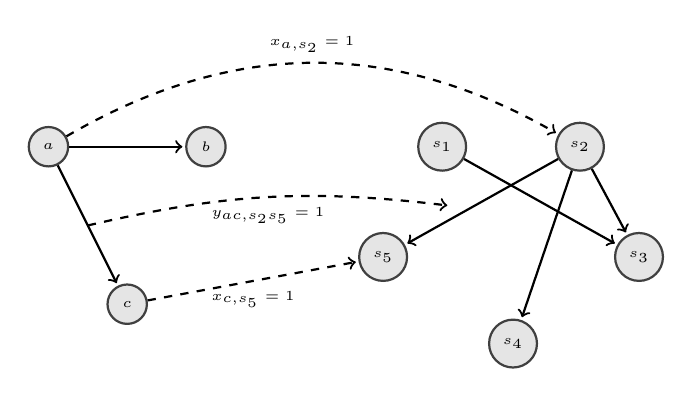
\begin{tikzpicture}[shorten >=1pt,->,scale=0.5]  
        \tikzstyle{node}=[circle,thick,draw=black!75,fill=black!10,minimum size=5mm]
        \tikzstyle{edge}=[draw, thick]
    	\begin{scope}
         \node [node] (a) at (0,4) {\tiny{$a$}};
         \node [node] (b) at (4,4) {\tiny{$b$}};
         \node [node] (c) at (2,0) {\tiny{$c$}};
         \path[edge] (a) to  (b);
         \path[edge] (a) to  (c);
            
         \node [node] (s1) at (10,4) {\tiny{$s_1$}};
         \node [node] (s2) at (13.5,4) {\tiny{$s_2$}};
         \node [node] (s3) at (15,1.2) {\tiny{$s_3$}};
         \node [node] (s4) at (11.8,-1) {\tiny{$s_4$}};
         \node [node] (s5) at (8.5,1.2) {\tiny{$s_5$}};

         \path[edge] (s1) to (s3);
         \path[edge] (s2) to (s3);
         \path[edge] (s2) to (s4);
         \path[edge] (s2) to (s5);
         
         \path[edge,dashed, bend left=30] (a) to  [above] node[font=\tiny] {$x_{a,s_2}=1$} (s2);

         \path[edge,dashed] (c) to  [below] node[font=\tiny] {$x_{c,s_5}=1$} (s5);

         \path[edge,dashed, bend left=10] (1,2) to  [below] node[font=\tiny] {$y_{ac,s_2s_5}=1$} (10.2,2.5);
         \end{scope}

      \end{tikzpicture}
\end{tabular}
   \caption{An illustration of mapping variables to overlay graph $g$ with coherence pattern $pat_u$.}
   \label{fig:Map_Var}
\end{center}
\end{figure}

Given the above variables, we need to define some constrains in order to check if pattern $cp_u$ is an induced subgraph of the selected nodes in projection graph $g$. 
To do so, we borrow constrains from \cite{lerouge15} to check if the pattern is an induced subgraph of the projection graph or not. 


\begin{itemize}
\item Every node of the pattern matches at most one unique node of the graph:

\begin{equation}
\sum_{k\in V_g}x_{i,k} \leq 1 \quad \forall i\in V_{pat_{u}}
\end{equation}

\item Every edge of the pattern matches at most one unique edge of the graph:

\begin{equation}
\sum_{kl\in E_g}y_{ij,kl} \leq 1 \quad \forall ij\in E_{pat_{u}}
\end{equation}

\item Every node of the graph matches at most one node of the pattern:

\begin{equation}
\sum_{i\in V_{pat_{u}}}x_{i,k} \leq 1 \quad \forall k\in V_g
\end{equation}

\item A node of pattern $cp_u$ matches a node of graph $g$ if an edge originating from the node of $cp_u$ matches an edge originating from the node of $g$:

\begin{equation}
\sum_{kl \in E_g}y_{ij,kl} =  x_{i,k}\textit{  }\forall k \in V_g, \textit{  }\forall ij \in E_{pat_{u}}
\end{equation}

\item A node of pattern $cp_u$ matches a node of graph $g$ if an edge targeting the node of $cp_u$ matches an edge targeting the node of $g$:

\begin{equation}
\sum_{kl \in E_g}y_{ij,kl} =  x_{j,l}\textit{  }\forall l \in V_g,\textit{  }\forall ij \in E_{pat_{u}}
\end{equation}

\item We need a constraint to extract \emph{induced} patterns. 
Pattern $cp_{u}$ is an induced subgraph of graph $g$ if $cp_{u}$ contains all possible edges that are present in $g$. 
So

\begin{equation}
\sum_{i \in V_{pat_{u}}}x_{i,k} + \sum_{j \in V_{pat_{u}}}x_{j,l} - \sum_{ij\in E_{pat_{u}}}y_{ij,kl} \leq 1
 \quad\textit{  }\forall kl\in E_g
\end{equation}
\end{itemize}

So far, our constrains check whether the pattern is an induced subgraph of the projection graph. 
But we must check if the pattern occurs in a subgraph of the projection graph that contains only selected sentence nodes for producing the summary. 
These constraints are not sufficient to check this. 
We define some more constraints to ensure that the pattern occurs in the selected nodes of the projection graph. 


\begin{itemize}

\item If sentences $s_{k}$ and $s_{l}$ are selected for the summary then the edge between them must be selected $(z_{kl}=1)$ as well.
\begin{equation}
 s_{k} \cdot s_{l}=z_{kl} \quad \forall k,l \in V_{g}
\end{equation}

\item Pattern $cp_u$ is present in the summary ($p_u=1$) if and only if one of its instances in the projection graph is included in the summary, i.e., some of the selected sentence nodes must be present in an instance of pattern $cp_{u}$.
$|V_{cp_{u}}|$ is the number of nodes in pattern $cp_{u}$, and $|E_{cp_u}|$ is the number of edges in pattern $cp_{u}$.
This constraint is shown below:

\begin{equation}
\underset{i \in V_{cp_u}}{\sum} \underset{k \in V_g}{\sum} s_k \cdot x_{i,k}+\underset{ij \in e_{cp_u}}{\sum} \underset{kl \in e_g}{\sum} z_{kl} \cdot y_{ij,kl} = p_{u}(|V_{cp_u}|+|E_{cp_u}|)
\end{equation}

\item If a sentence is selected then it has to match a node of at least one of the patterns:

\begin{equation}
\sum_{cp_{u} \in P} \sum_{i \in V_{cp_{u}}} x_{i,k} \geq s_{k} \quad \forall k \in V_{g}
 \end{equation}
\end{itemize}

Now we can set up our experiments to evaluate our enhanced  summarization system by coherence patterns. 

\paragraph{Data. }
We evaluate our model on two datasets:  \emph{PLOS Medicine} and \emph{DUC}. 

\textbf{PLOS Medicine. } 
This dataset contains $50$ scientific articles.  
We are motivated to evaluate our model on scientific articles because of the growth in scientific outputs in different fields that makes the task of automatic summarization imperative. 
Automatic summarizers assist researchers to have an informative and coherent gist of long scientific articles. 
Moreover, scientific articles consist of different sections that make the task roughly similar to \mbox{multi-document} summarization. 
The reason that we selected this dataset is that articles in this dataset are accompanied by summaries written by editors of the month. 
Editors' summaries have a broader perspective than abstracts of articles.  
We use editor's summaries as gold summaries for our evaluation goal.
This is dataset $D$  in our formulation.

Based on this assumption that abstracts of scientific articles are similar in style to coherent summaries, 
we use a dataset of abstracts if scientific articles in the \mbox{bio-medicine} field to mine coherence patterns and compute their weights.   
We use $700$ scientific articles from the PubMed\footnote{\url{http://www.ncbi.nlm.nih.gov/pmc/tools/ftp/}} corpus where articles do not overlap with articles in PLOS Medicine dataset. 
This dataset of abstracts is dataset $H$ in our formulation.


\textbf{DUC. } 
The DUC 2002 dataset has been annotated for the Document Understanding Conference 2002. 
It contains $567$ news articles for summarization. 
Every article is accompanied by at least two gold summaries.
This is dataset $D$ in our formulation and we use this dataset for the evaluation purposes. 
We use all ($300$) DUC 2005 human summaries to mine coherence patterns and to calculate their weights. 
This is dataset $H$ in our formulation.
% DUC 2002 articles are shorter than \emph{PLOS Medicine}\ articles (25 vs.\ 154 sentences average\ length). 


\paragraph{Model Configuration. }
In the preprocessing phase of scientific articles, we extract texts of articles by removing all figures, tables, references and \mbox{non-alphabetical} characters.
For both datasets, we use the Stanford parser \cite{klein03b} to  pars sentences. 
We employ the Brown coherence toolkit \cite{elsner11b} to convert  parse trees into entity grids \cite{barzilay08}. 
These then are transformed into entity graphs. 
We use gSpan \cite{yanxifeng02} to extract all coherence patterns from the projection graphs in $gs_H$. 
We use coherence patterns with $3$ and $4$ nodes, referred to as $CP_3$ and $CP_4$, respectively, due to patterns with a large number of nodes rarely occur in projection graphs.
We compute the weight of each pattern by considering the frequency of coherence patterns of the same size. 
Then, the importance values of sentences and the coherence patterns with their weights are used in the optimization phase. 
The optimization is formulated as Mixed Integer Programming (MIP), which deals with quadratic constraints. 
We use Gurobi \cite{gurobi14} to solve the MIP optimization problem.
We determine the best values for $\lambda_{I}$, $\lambda_R$, and $\lambda_{c}$ on the development sets.
\textbf{SIZE OF DEV SET? SPLIT PRECENTAGE?}
$\lambda_{I}=0.4$, $\lambda_R=0.3$, and $\lambda_{c}=0.3$ are the best weights for the \emph{PLOS Medicine}\ development set. Weights for the DUC 2002 development set are $\lambda_{I}=0.5$, $\lambda_R=0.2$ and $\lambda_{c}=0.3$.
When a summary is produced, we replace all pronouns with their antecedences using the pronoun resolution system proposed by \newcite{martschat13}. 
we limit the length of summaries to $5$ sentences,  when we compare our system with the state-of-the-art systems on PLOS Medicine. 
However, since the word length limit of a summary makes more sense than the sentence length limit of a summary, we also compare our systems when the length of a summary is restricted to the average length of editor's summaries in the dataset ($750$ words). 
                                                                                       
% In Figure 3 we overlay the projection graph from Figure 2, ii with the coherence pattern from Figure 1, i. 
% This results in three instances of this coherence pattern. 
% However, we select only one since we simultaneously optimize for importance and non-redundancy. 

% % We want to incorporate coherence patterns as a coherence measure, and build a model which tightly connects coherence, non-redundancy and importance.
% % To achieve this, we deal with the graph matching problem.

% We use the mined patterns to extract sentences from the input document of PLOS Medicine to create a coherent summary. 
% We extract sentences, if the connectivity among nodes in their projection graph matches the connectivity among nodes in a coherence pattern. 

% The key idea of this paper is to apply coherence patterns to long scientific articles to extract (possibly) non-adjacent sentences which, however, are already coherent. 

% Then we apply the most frequent coherence patterns to input documents, i.e. long scientific articles from bio-medicine (PLOS Medicine dataset), extract corresponding sentences to generate coherent summaries, and evaluate them by comparing with summaries written by a PLOS Medicine editor. 
% Figure 1 illustrates the extraction of sentences from an input document (Figure 1, (ii)) which constitute a coherence pattern (Figure 1, (i)).  
% If we overlay the input document with coherence patterns and extract the sentences which constitute those patterns, then the extracted sentences are al- ready coherent. We also take into account importance and non-redundancy. We capture all three factors in an objective function maximized by Mixed Integer Programming (MIP).


\paragraph{Results. }
We evaluate our model in two ways. 
First, we use ROUGE scores to compare our summarizer with other models. 
Second, we explicitly evaluate the coherence of summaries by human judgements.

\textbf{ROUGE Assessment. }
The ROUGE score \cite{linchinyew04} is a standard evaluation metric for automatic text summarization. 
It principally measures word overlaps between gold summaries (usually generated by humans) and summaries produced by a model. 
ROUGE 1, ROUGE 2 and ROUGE SU4 are three versions of ROUGE that are popularly reported for comparing different summarization systems.  
We refer interested readers to  \newcite{graham15} for more explanations about evaluation metrics for the summarization task. 
We compare following summarization systems: 

\begin{itemize}
	\item \emph{Random}: that selects sentences randomly;

	\item \emph{Lead}: that includes the top n\% of the sentences of a document

	\item \emph{Maximal Marginal Relevance (MMR)} \cite{carbonell98}: which uses a \mbox{trade-off} between relevance and redundancy; 

	\item \emph{Text-Rank} \cite{mihalcea04b}: represents an input document by a graph whose nodes represent sentences and edges are weighted by cosine similarity between sentences; 
	\textbf{Then?}

	\item \emph{$E_{Coh}$}\ \cite{parveen15a}: that uses the entity graph of an input document to encode \mbox{entity-based} relations among sentences. 
	It uses the outdegree of sentence nodes in the unweighted projection graph of an input document, as the coherence measure of each sentence.

	\item \emph{$T_{Coh}$}\ \cite{parveen15b}: that uses topical graphs instead of entity graphs to encode topical relations among sentences. 
	Topical graphs are bipartite graphs consisting of two sets of nodes: sentences and topics. 
	The outdegree of each sentence in weighted projection graphs are taken as the coherence measure of the sentence.

	\item \emph{Mead} \cite{radev04b}: that assigns a score to each sentence of a document using three other scores: the centroid score (which is a measure of the centrality of a sentence to the overall topic of a document), the position score (which  decreases linearly as the sentence gets farther from the beginning of a document), and the \mbox{overlap-with-first} score (which is the inner product of the \mbox{TF*IDF-weighted} vector representations of a sentence and the first sentence (or title, if there is one) of an input document. 
	MEAD discards sentences that are too similar to other sentences (based on a cosine similarity). 
	Any sentence that is not discarded due to high similarity and which gets a high score (within the specified compression rate) is included in the summary. 
	% All three features do not take care of the coherence of a summary as they do not have any notion of the order and the structure of a summary .

	\item \emph{$CP_3$}: that is our summarization approach where it uses \mbox{3-node} subgraphs as coherence patterns

	\item \emph{$CP_4$}: that is our summarization model where it uses \mbox{4-node} subgraphs as coherence patterns

	\item  \emph{Upper Bound} represents maximum ROUGE scores
	that can be achieved in extractive summarization a dataset. 
	It is calculated by considering the whole input document as a summary.
	
\end{itemize}


Table \ref{table:plos_5len_editor} reports ROUGE scores of different systems on the \emph{PLOS Medicine} dataset. 
%
\begin{table}[!ht]
\centering
\small
\begin{tabular}{@{}l|c|c@{}}
\hline
Systems & R-SU4 & R-2\\
\hline
\textbf{Baselines}&  & \\
Lead & 0.067 &  0.055  \\
Random &  0.048  & 0.031  \\
MMR & 0.069 &  0.048  \\
TextRank & 0.068  & 0.048  \\
\textbf{State-of-the-art}&  & \\\hline
$E_{Coh}$ & 0.131& 0.098 \\
$T_{Coh}$\ & 0.129 & 0.095  \\
Mead & 0.084 & 0.068 \\
\textbf{Our Model} & & \\\hline
$\mathbf{CP_3}$ & \textbf{0.135} & \textbf{0.103} \\
\hline
\end{tabular}
\caption{\emph{PLOS Medicine}, editor's summaries with \textbf{5 sentences}.}
\label{table:plos_5len_editor}
\end{table}



Table \ref{tab:plos_rougesu4} shows the performance of different systems with $750$ words limit for a summary when editor's summaries are taken as gold standard. 
We calculate different variations of ROUGE-2 and ROUGE-SU4. 
These variations demonstrate the effect of stop words and stemming in ROUGE calculation.
For sake of brevity, we use the notation ``SW'' to refer to stop words and ``SM'' to refer to word stemming.  
``SW--'' shows that stop words are not taken into account in ROUGE calculation; ``SW+'' is the opposite. 
``SM--'' shows that Porter Stemmer is not applied to summaries in ROUGH calculation, ``SM+'' is its opposite. 
 
Our models achieves the best performance in comparison to other examined systems with respect to all variations of ROUGE. 
When we integrate coherence patterns with three nodes into the summarizer, $CP_3$, it significantly outperforms $E_{Coh}$ that uses the outdegree of sentence nodes as the coherence feature. 
This result confirms our intuition that the outdegree of nodes in the projection graph of a document is not a powerful representative for coherence of selected sentences for a summary. 
$CP_3$ works better than $E_{Coh}$ basically because our coherence patterns capture the connectivity style among selected sentences for a summary, whereas
the outdegree measures to what extend a sentence is connected to other sentences  in a document, rather than a summary. 
Moreover, the outdegree does not capture how sentences should be connected to have a more coherent summary. 
% We compute statistical significance between \emph{$E_{Coh}$}\ and \emph{$CP_3$}\ on both scores, ROUGE-SU4 is significantly different by 95\%. ROUGE-2 is significantly different by 99\%.

\begin{table*}[!ht]
\centering
\small
\begin{tabular}{@{}l|r@{}l|r|r|r||r@{}l|r|r|r@{}}
\hline
\emph{PLOS Medicine}& SW--& & SW-- & SW+ & SW+& SW-- & & SW-- & SW+ & SW+ \\
Editor's summaries  & SM-- & & SM-- &  SM+ & SM-- &  SM+  & & SM-- &  SM+  & SM-- \\\hline
&& \multicolumn{4}{c||}{ROUGE SU4 ($\ast p<.05$)} & \multicolumn{4}{c}{ROUGE 2 ($\ast p<.01$)}\\\hline
\textbf{Upper Bound} & 0.423 & & 0.354 &0.519 &0.470  & 0.344 & & 0.304 & 0.430 & 0.399  \\\hline
% \multicolumn{9}{r}{\textbf{Baselines}}\\\hline
 \textbf{Baselines} & & & & & & & & & &\\
Random &  0.140& & 0.113 & 0.169  & 0.153 &  0.102 & & 0.088 & 0.125 & 0.116 \\
Lead & 0.191 & & 0.158 & 0.246 & 0.222  & 0.158 & & 0.140 &0.185 &0.171   \\
MMR & 0.183& & 0.149 & 0.240 & 0.215 & 0.141 & & 0.125 & 0.171 &0.157 \\
TextRank & 0.148& & 0.104 & 0.161 & 0.159 & 0.115 & & 0.084 &0.126 & 0.118\\\hline
\textbf{State-of-the-art} & & & & & & & & & & \\
Mead & 0.197 & & 0.165 & 0.246 & 0.222& 0.156 & &0.139 & 0.186 & 0.172 \\
$E_{Coh}$ & 0.204&* & 0.167 & 0.254& 0.228 &0.160 &* & 0.145 &0.187 & 0.173\\
$T_{Coh}$\ & 0.195 & &0.161 & 0.231 &0.206 & 0.157 &  & 0.140 &0.169 & 0.165 \\\hline
\textbf{Our Model} & & & & & & & & & &\\
$CP_3$ &0.215& * &0.178& 0.268& 0.241& 0.172 & * & 0.153 & 0.200 &0.184 \\
$CP_4$ & \textbf{0.218}& & \textbf{0.179} & \textbf{0.270} & \textbf{0.245}  & \textbf{0.175} & & \textbf{0.156} & \textbf{0.201} & \textbf{0.187} \\
\hline
\end{tabular}
\caption{ROUGE scores on \emph{PLOS Medicine} with \textbf{750 words}.}
\label{tab:plos_rougesu4}
\end{table*}

When we integrate coherence patterns with four nodes, $CP_4$, the summarizer works slightly better than $CP_3$ confirming that large subgraphs capture more information about the connectivity style of nodes in a projection graph and therefore the coherence of sentences.  
However, this improvement is not statistically significant. 
4-node patterns are less likely to occur than 3-node patterns because coherence patterns should occur in a subgraph of the projection graph that contains only selected nodes. 

$CP_3$ also outperforms \emph{Mead} as one of the state-of-the-art summarization systems. 
On average summaries produced by \emph{Mead} contains less number of sentences than summaries produced by $CP_3$ (17.5 vs 27.2 sentences per summary).
This shows that \emph{Mead} selects longer sentences in comparison to \emph{$CP_3$}. 
Long sentences are more complex and less readable. 
They also contain more irrelevant entities than shorter sentences.

% The other interesting impact of our coherence pattern is that it makes the summarizer extract sentences almost from different sections of scientific articles.  
% \emph{$CP_3$} extracts sentences mainly from Introduction ($32.5$\%) and Method ($38.5$\%), but also a considerable number of sentences from Results ($17.67$\%) and Discussion ($11.33$\%). 
% This is similar to the distribution of selected sentences by \emph{TextRank} and \emph{MMR}.
% On there hand, \emph{Lead}  extracts only from Introduction ($80.59$\%) and Method ($19.41$\%). 
% \emph{Mead} extracts maximum sentences from the beginning of the document due to its position feature.
% $E_{Coh}$ and $T_{Coh}$ are also biased to extract sentences from the beginning of a document mainly because the outdegree of sentences at the beginning of the document are potentially greater than other sentences.  
% Our coherence patterns make the summarizer unbiased to positions of sentences in a document because of two reasons. 
% First, unlike outdegree, our patterns do not consider each sentence individually.  
% They are style-based and model the connectivity style among sentences. 
% Second, our coherence patterns are graph-based, so they can capture long distant connections between sentences, which may occur across sections, as well as short distant relations, which occur within sections.    
% \begin{table}[!h]
% \centering
% \small
% \begin{tabular}{l|l|l|l|l}
% \hline
% Systems & Introduction & Method & Results & Discussions\\\hline

% Lead & 80.59 & 19.41 & 0 & 0\\
% TextRank & 25.67 & 48.21 & 16.10 & 10.02\\
% Mead & 43 & 20.7& 21&15.3 \\
% MMR & 29.65 & 35.41 & 15.49 & 19.45\\
% $E_{Coh}$ & 31.49 & 40.30 & 15.00 & 13.21 \\
% $CP_3$ & 32.50 & 38.5 & 17.67 & 11.33\\
% \hline
% \end{tabular}
% \caption{Sectional distribution (\%) of summaries.}
% \label{table:section_dist}
% \end{table}


\textbf{DUC. }
Table \ref{table:duc2002_res} shows the results on DUC 2002 for well-performed  systems in the previous experiment. 
In addition, we compare our model to \emph{NN-SE} that utilizes a neural network hierarchical document encoder and an \mbox{attention-based} extractor to extract sentences from a document for a summary \cite{chengjianpeng16}.

ROUGE scores of our approach on this dataset surpass the scores of baselines and state-of-the-art systems. 
This shows that our system performs well even in a different domain and with considerably shorter input documents. 
Our model outperforms the \emph{NN-SE} system, because our model explicitly takes into account the connectivity of selected sentences in the sentence extraction phase. 

% There is no significant difference between the ROUGE scores of using $CP_3$ and $CP_4$ on DUC 2002 as well. 


\begin{table}[!ht]
\centering
\small
\begin{tabular}{@{}l|c|c|c@{}}
\hline
Systems & R-1 & R-2 & R-SU4\\\hline
\textbf{Baselines}  & & &\\
Lead & 0.459 & 0.180 & 0.201\\
TextRank & 0.470 & 0.195 & 0.217\\
DUC 2002 Best & 0.480 & 0.228 & \\\hline
\textbf{State-of-the-art}  & & &\\
Mead & 0.445 & 0.200 & 0.210\\
$E_{Coh}$ & 0.485 & 0.230 & 0.253 \\
$T_{Coh}$\ & 0.481 & 0.243 & 0.242 \\
NN-SE & 0.474 & 0.23 & \\\hline
\textbf{Our Model} & & & \\
$CP_3$ & \textbf{0.490} & \textbf{0.247} & \textbf{0.258}\\
\hline
\end{tabular}
\caption{ROUGE scores on DUC 2002.}
\label{table:duc2002_res}
\end{table}



\textbf{Coherence Assessment. } 
Here we perform a qualitative evaluations on the summaries produced by different systems. 
We follow \newcite{parveen15b} and exclusively assess the coherence aspect of summaries by asking human assessors to rank summaries that are generated by different systems. 
% \newcite{haghighi09a}, \newcite{celikyilmaz10} and \newcite{christensen13} evaluate the overall summary quality by asking human subjects to rank system generated summaries. 
To do so, we ask four NLP colleague of us (one PostDoc, two PhD students and one Masters student) to rank summaries if four different systems for ten different articles. 
The most coherent summary gets rank $1$, the second best gets rank $2$, the third best gets rank $3$, and the worst gets rank $4$.
The four summarization systems are
\emph{$CP_3$}, \emph{$E_{Coh}$}, \emph{Text\-Rank}, and \emph{Lead}.

We apply the Kendall concordance coefficient (W) \cite{siegel88} in order to measure the agreement between the human assessors in ranking the examined summaries. 
We calculate Kendall's W for every scientific article which is given to the human subjects. 
Then, we calculate the average of Kendall's W of scientific articles. 
The average Kendall's W is $0.6725$,  which indicates a high level of agreement between human subjects.
With W $= 0.6725$ the correlation between the human assessors is high. 
Applying the $\chi^2$ test shows that W is significant at least at the 95\% level indicating that the ranks provided by the human assessors are reliable and informative.

Table \ref{table:coherence_assessment} shows the overall average rankings summaries produced by a system received by human judges. 

\begin{table}[!ht]
\centering
\small
\begin{tabular}{l|c}
\hline
System &  Average Human Score\\
\hline
TextRank & 3.950\\
$E_{Coh}$ & 2.325\\
$\mathbf{CP_3}$ & \textbf{1.875} \\
Lead & 1.625\\
\hline
\end{tabular}
\caption{The average human scores. Lower is better. (\emph{PLOS Medicine}) }
\label{table:coherence_assessment}
\end{table}

As expected, \emph{Lead} obtains the best overall average rank because it extracts adjacent sentences from the beginning of the document. 
Hence, these summaries are as coherent as the author intends them to be, but they are not informative.
\emph{$CP_3$} outperforms $E_{Coh}$ and $TextRank$ and follows $LEAD$ confirming that summaries that generated using our coherence patterns are perceived more coherent than those of other system. 



\section{Conclusions}
\label{sec:conclusions}
In this chapter, we challenged the average outdegree metric that is heuristically defined so that documents whose projection graphs have higher average outdegrees are more coherent. 
We showed that the average outdegree of nodes in a projection graph is not sufficient to capture the connectivity style of nodes and consequently the perceived coherence of the corresponding document. 
Instead, we proposed novel coherence patterns that capture the entity-based connectivity style of sentences in documents. 
We employed unweighted projection graphs of documents in a corpus to encode the connectivity style of sentences in documents.  
Then by applying a subgraph mining algorithm to all projection graphs of all documents, we mine all occurring subgraphs in these graphs as coherence patterns. 
We use the frequency of each coherence pattern in a projection graph as a representative feature of the connectivity style of nodes in the projection graph and consequently, a representative feature of the perceived coherence of the corresponding document. 

We evaluated our coherence patterns in two applications: readability assessment and extractive \mbox{single-document} summarization. 
In the former, we observed that frequencies of some coherence patterns are positively and some other negatively correlated with readability scores assigned by human judges. 
Positively correlated patterns mostly depict this intuition in texts that a sentence introduces some entities and its subsequent sentences elaborate each of them.  
Negatively correlated patterns roughly remind us the linear chain pattern in linguistics where a sentence is located between two unrelated sentences to make them connected. 
Although this pattern is useful but if it occurs too frequently in a document then it hurts the coherence of the document. 
Our experiments showed that 4-node subgraphs have a better predictive power than  3-node subgraphs in ranking documents with respect to their readability. 
We believe that this is mainly because large coherence patterns have more capacity than small ones for encoding the connectivity style of nodes in projection graphs. 

In the summarization task, we examined our coherence patterns by integrating them into an existing summarization system that is developed on the entity graph representation of documents. 
This task was challenging  because we had to model the existence of our coherence patterns in a summary by defining several new constraints in linear programming.  
The results of our experiments on DUC 2002 as an standard dataset for summarization and PLOS Medicine as a corpus of scientific articles show that our coherence patterns improve the performance of the summarizer with respect to ROUGE and human evaluation. 


The key message of this chapter is that in order to capture the connectivity style of sentences in  a document, which is encoded via the projection graph of the document, coherence patterns that are obtained automatically by applying a subgraph mining algorithm to projection graphs are more useful than average outdegree that is designed heuristically. 
Coherence patterns capture coherence beyond the level of sentences, and take a sentence in its connections with other sentences. 
Our \mbox{data-driven} approach to coherence patterns enables us to extract patterns from documents that are provided for an application and collected in a dataset. 

We observed that 4-node subgraphs are better coherence patterns than 3-node subgraphs. 
However, more investigation is requited to be performed on how the size of subgraphs influences the performance of the model. 
The entity graph does not include mentions that are semantically related but are not correferent. 
It would be interesting to see if entity graphs will have enriched by more  connections, the our coherence patterns still work. 
We follow these points in the next chapter of this thesis.  
However, we see other directions for future work for this chapter. 

\textbf{Future Work}











% \section{Related Work}
% \label{sec:related_work}

% There is a research tradition developing metrics for readability and using these metrics to quantify how difficult it is to understand a
% document. 
% Shallow features such as word, sentence and text length, which only capture superficial properties of a text, have been used traditionally \cite{flesch48,kincaid75}. \newcite{declercq14} use traditional shallow features and apply these to a new corpus annotated with two different methodologies. 
% However, some studies indicate that shallow features do not precisely predict the readability of a text \cite{fenglijun09,petersen09}. Later studies introduce deeper (more
% semantic) features such as those obtained by language models \cite{siluo01,collins-thompson04} and syntactic features like the number of NPs in sentences or the height of the sentence's parse tree \cite{schwarm05,heilman07}. 
%  \newcite{barzilay08} propose an entity-based coherence model which operationalizes some of the intuitions behind the centering model \cite{grosz95}.  
%  Although this model works well on the sentence ordering and summary coherence rating tasks, it does not work well for readability assessment. 
%  Only when combining the entity grid with features taken from \newcite{schwarm05} the entity grid performs competitively.

% While most of these studies predict the readability level of documents, \newcite{pitler08} present a new readability dataset with \textit{Wall Street Journal} articles, where each article is assigned human readability ratings. 
% They analyze the correlation between different readability features and human readability scores. 
% They show no correlation between entity-transition features and readability scores. 
% In contrast to them we are able to report a statistically significant correlation between some entity-based features and human readability ratings.

% They use coherence features based on entity transitions in the entity grid \cite{barzilay08}. 
% None of these features are strongly correlated with the readability ratings. While these features are intended to capture entity-based coherence, entity transitions in isolation seem to be too weak to actually do so. 
% \newcite{miltsakaki00} show that for having a well-written text, the author should avoid to concatenate sentences without sharing any entity.

% Summarizing scientific articles is as difficult as multi-document summarization because scientific articles are tend to be long and the important information is spread all over the article unlike information in news articles \cite{teufel02}.

% There are various approaches for summarizing scientific articles. Citations have been used by many researchers for summarization in this domain \cite{elkiss08,mohammad09,qazvinian08,abu-jbara11}. \newcite{nanba00} develop rules for categorizing citations by analyzing the citation sentences. \newcite{newmanmark01} analyzes the structure using a citation network. Similarly, \newcite{siddharthan07} discover scientific attributions using citations. Discourse structure (but not necessarily coherence) has been used by \newcite{teufel02}, \newcite{liakata13} and others for summarizing scientific articles.

% Several state-of-the-art extractive summarization systems implement summarization as maximizing an objective function using constraints.
% \newcite{mcdonald07} interprets text summarization as a global inference problem, where he is maximizing the importance score of a summary by considering the length constraint. Similarly, various approaches for summarization are based on optimization using ILP  \cite{gillick09,nishikawa10,galanis12,parveen15a}.

% Until now, only few works have considered coherence while summarizing scientific articles. \newcite{abu-jbara11} work on citation based summarization. They preprocess the citation sentences to filter out irrelevant sentences or sentence fragments, then extract sentences for the summary. Eventually, they refine the summary sentences to improve readability.
% % They filter out unsuitable sentences using classification and extract
% % the scope of the reference from the citation sentences, then extract important sentences using LexRank \cite{erkan04}. 
% \newcite{jha15} consider Minimum Independent Discourse Contexts (MIDC) to solve the problem of non-coherence in extractive summarization.
% However, none of them deals with the problem of coherence within the task of sentence selection. Sentence selection and ensuring the coherence of summaries
% are not tightly integrated in their techniques. They model coherence in summarization by only considering adjacent sentences.

% There are few methods \cite{hirao13,parveen15a,gorinski15} which integrate coherence in optimization.
% These methods do not take into account the overall structure of the summary. Unlike earlier methods, we incorporate coherence patterns in optimization.


